%----------------------------------------------------------------------------------------
%	PACKAGES AND OTHER DOCUMENT CONFIGURATIONS
%----------------------------------------------------------------------------------------

\documentclass[paper=a4, fontsize=11pt]{scrartcl} % A4 paper and 11pt font size
\usepackage[a4paper, left=2.5cm, right=2cm, top=2cm, bottom=2cm]{geometry}
\linespread{1.2}

\usepackage[utf8]{inputenc}
\addtokomafont{disposition}{\rmfamily}
\usepackage{polski} % Język polski/hyphenation
\usepackage{amsmath,amsfonts,amsthm} % Math packages
\usepackage{indentfirst}
\usepackage{graphicx}
\usepackage{caption}
\usepackage{flafter}
\usepackage{flexisym}
\usepackage{listings}
\usepackage{color}
\usepackage{subcaption}
\usepackage{enumitem}
\usepackage{float}
\usepackage{tabularx}


\def \thesis {Aplikacja uczenia maszynowego metodą SVM}
\def \author {Pavlo Boidachenko}
\def \department {Wydział Fizyki, Astronomii i Informatyki Stosowanej}

\usepackage{sectsty} % Allows customizing section commands
%\allsections{\mdseries\itshape} % Make all sections centered, the default font and small caps

\usepackage{fancyhdr} % Custom headers and footers
\pagestyle{fancy} % Makes all pages in the document conform to the custom headers and footers
\fancyhead[L]{\textbf{Praca licencjacka:} \thesis} % No page header - if you want one, create it in the same way as the footers below
\fancyhead[C]{}
\fancyhead[R]{}
\fancyfoot[L]{\author} % left footer
\fancyfoot[C]{\thepage} % center footer
\fancyfoot[R]{} % right footer
\renewcommand{\headrulewidth}{0.3pt} % Remove header underlines
\renewcommand{\footrulewidth}{0.3pt} % Remove footer underlines
\setlength{\headheight}{14.06pt} % Customize the height of the header

% bibliography
\usepackage[style=alphabetic,sorting=nyt,sortcites=true,autopunct=true,babel=hyphen,hyperref=true,abbreviate=false,backref=true,backend=biber,citestyle=numeric]{biblatex}
\addbibresource{ref.bib}
\defbibenvironment{bibliography}
{\list
     {\printtext[labelnumberwidth]{%
      \printfield{labelprefix}%
      \printfield{labelnumber}}}
     {\setlength{\labelwidth}{\labelnumberwidth}%
      \setlength{\leftmargin}{\labelwidth}%
      \setlength{\labelsep}{\biblabelsep}%
      \addtolength{\leftmargin}{\labelsep}%
      \setlength{\itemsep}{\bibitemsep}%
      \setlength{\parsep}{\bibparsep}}%
      \renewcommand*{\makelabel}[1]{\hss##1}}
  {\endlist}
  {\item}



% listing settings
\definecolor{mygreen}{rgb}{0,0.6,0}
\definecolor{mygray}{rgb}{0.5,0.5,0.5}
\definecolor{mymauve}{rgb}{0.58,0,0.82}

\lstset{ 
  backgroundcolor=\color{white},   % choose the background color; you must add \usepackage{color} or \usepackage{xcolor}; should come as last argument
  basicstyle=\footnotesize,        % the size of the fonts that are used for the code
  breakatwhitespace=false,         % sets if automatic breaks should only happen at whitespace
  breaklines=true,                 % sets automatic line breaking
  captionpos=b,                    % sets the caption-position to bottom
  escapeinside={(*@}{@*)},
  commentstyle=\color{mygreen},    % comment style
  extendedchars=false,              % lets you use non-ASCII characters; for 8-bits encodings only, does not work with UTF-8
  frame=single,	                   % adds a frame around the code
  keepspaces=true,                 % keeps spaces in text, useful for keeping indentation of code (possibly needs columns=flexible)
  keywordstyle=\color{blue},       % keyword style
  language=C++,                 % the language of the code
  morekeywords={*,...},            % if you want to add more keywords to the set
  rulecolor=\color{black},         % if not set, the frame-color may be changed on line-breaks within not-black text (e.g. comments (green here))
  showspaces=false,                % show spaces everywhere adding particular underscores; it overrides 'showstringspaces'
  showstringspaces=false,          % underline spaces within strings only
  showtabs=false,                  % show tabs within strings adding particular underscores
  stepnumber=2,                    % the step between two line-numbers. If it's 1, each line will be numbered
  stringstyle=\color{mymauve},     % string literal style
  tabsize=2,	                   % sets default tabsize to 2 spaces
  title=\lstname                   % show the filename of files included with \lstinputlisting; also try caption instead of title
}

\numberwithin{equation}{section} % Number equations within sections (i.e. 1.1, 1.2, 2.1, 2.2 instead of 1, 2, 3, 4)
\numberwithin{figure}{section} % Number figures within sections (i.e. 1.1, 1.2, 2.1, 2.2 instead of 1, 2, 3, 4)

\renewcommand{\thetable}{\Roman{table}}

\setlength\parindent{10pt} % Removes all indentation from paragraphs - comment this line for an assignment with lots of text

\newcommand{\horrule}[1]{\rule{\linewidth}{#1}} % Create horizontal rule command with 1 argument of height

\newcommand*{\captionsource}[2]{% caption with source for images
  \caption[{#1}]{%
      #1}
    %\\\hspace{\linewidth}%
    Źródło: #2%
  %
}

\newcommand{\norm}[1]{\left\lVert#1\right\rVert}

%Other packages
\usepackage{multirow}
\usepackage{url}
\usepackage{bm}
\usepackage{xcolor}
\definecolor{Black}{RGB}{0,0,0}
\definecolor{Red}{RGB}{255,0,0}
\definecolor{Blue}{RGB}{0,0,255}
\definecolor{Green}{RGB}{0,255,0}
\definecolor{Gray}{RGB}{45,45,45}
\definecolor{linkcol}{RGB}{57,0,155}
\usepackage[unicode, pdftex, colorlinks=true, urlcolor=Gray, linkcolor=Gray, citecolor=Gray]{hyperref}

\usepackage{tocloft}
\renewcommand{\cftsecleader}{\cftdotfill{\cftdotsep}}

\begin{document}

\thispagestyle{empty}
\begin{titlepage}
    \begin{center}
        \Large \textbf{Uniwersytet Jagielloński w Krakowie}\vspace{0.2cm}\\ \department\\
        \vspace*{1cm} 
        \vspace{3cm}
        \Large
        \textbf{\author}\\\vspace{0.5cm}
        \normalsize Nr albumu: 1124969\\
        \vspace{2cm}
        \Huge
        \textbf{\thesis}

        \vspace{1.5cm}
        \normalsize
        Praca licencjacka\\
        na kierunku informatyki\\ \vspace{0.15cm}
        \vfill
        \vspace{2cm}
        \begin{minipage}{1\textwidth}
            \begin{flushright}
                Praca wykonana pod kierunkiem\\
                dr Grzegorz Surówka\\
                Zakład Technologii Informatycznych 
            \end{flushright}
        \end{minipage}
        \vspace{2cm}
        \begin{center}
            Kraków 2019
        \end{center}
    \end{center}

\end{titlepage}

\newpage 
 \thispagestyle{empty}
\vspace{2.5cm}
\begin{flushleft}
\large \textbf{Oświadczenie autora pracy}\vspace{0.6cm}\\
\end{flushleft}

\noindent Świadom odpowiedzialności prawnej oświadczam, że niniejsza praca dyplomowa została napisana przeze mnie samodzielnie i nie zawiera treści uzyskanych w sposób niezgodny z obowiązującymi przepisami.\\

\noindent Oświadczam również, że przedstawiona praca nie była wcześniej przedmiotem procedur związanych z uzyskaniem tytułu zawodowego w wyższej uczelni.
\vspace{2cm}
\begin{center}
    \begin{tabular}{lr}
        ................................~~~~~~~~~~~~~~~~~~~~~~~~~~~~~~~~~~~~~~&
        .......................................... \\
        {~~~~Kraków, dnia} & {Podpis autora pracy~~~~}
    \end{tabular}
\end{center}
\vspace{5cm}
\begin{flushleft}
    \large \textbf{Oświadczenie kierującego pracą}
\end{flushleft}

\noindent Potwierdzam, że niniejsza praca została przygotowana pod moim kierunkiem
i~kwalifikuje się do przedstawienia jej w postępowaniu o nadanie tytułu zawodowego.
\vspace{2cm}
\begin{center}
    \begin{tabular}{lr}
        ................................~~~~~~~~~~~~~~~~~~~~~~~~~~~~~~~~~~~~~~&
        ............................................ \\
        {~~~~Kraków, dnia} & {Podpis kierującego pracą~~}
    \end{tabular}
\end{center}
\vfill

\newpage
\tableofcontents

\newpage
\section{Wstęp} % SECTION
\subsection{Motywacja}
    \par W aktualne czasy temat Uczenia Maszynowego jest popularny\ref{fig:google-trends-ml}
    jak nigdy do tego.  Projekty z użyciem Uczenia Maszynowego pozwalają na tworzenie aplikacji
    które jeszcze 10 lat temu trudno było wyobrazić.

    \begin{figure}[H]
        \begin{center}
            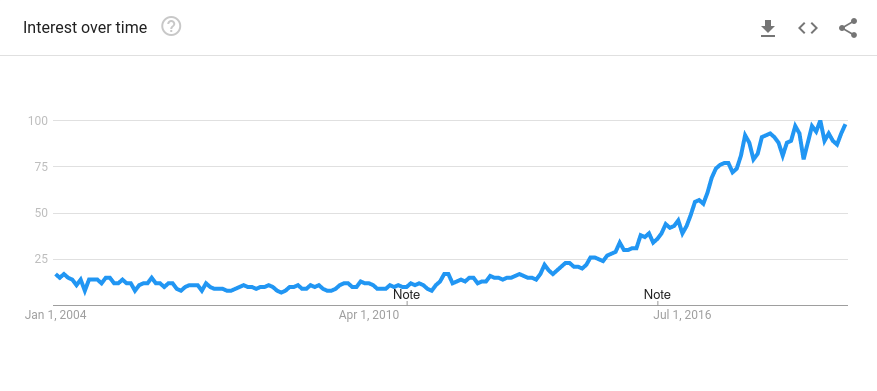
\includegraphics[scale=0.5]{./img/google-trends-ml.png}
            \captionsource{Machine Learning trends}{Google Trends}
            \label{fig:google-trends-ml}
        \end{center}
    \end{figure}

    \par Rozpowszechnienie Uczenia Maszynowego również spowodowało i moje zainteresowanie
    tematem.  Z tego powodu dla swojej pracy licencjackiej wybrałem temat: Aplikacja uczenia
    maszynowego metodą SVM. Po zakończeniu pracy spodziewam się podwyższyć swoją kompetencje w
    dziale Uczenia Maszynowego.
    \par SVM jest atrakcyjną metodą nienadzorowanego Uczenia Maszynowego, specjalną własnością
    której jest ciągłe zmniejszenie błędu i maksymalizacja marginesu, co pozwala nie tylko
    odseparować klasy, a odseparować ich z maksymalnym marginesem. Z czego wynika większa
    dokładność modelu na nowych danych.

\subsection{Cel}
    \par Celem mojej pracy licencjackiej jest stworzenie oprogramowania pozwalającego na
    generowanie modeli używając Maszyny wektorów wspierających\textit{(ang. Support Vector
    Machine, SVM)} z graficznym interfejsem użytkownika.  Program będą mogli użyć osoby
    potrzebujące szybko przetrenować kilka modeli, przetestować ich dla różnych parametrów,
    zwizualizować dane. Program ma na celu ułatwienie pracę z Maszyną wektorów wspierających
    poprzez graficzny interfejs użytkownika oparty na bibliotekę QT. Część funkcjonalna
    programu jest oparta o bibliotekę LIBSVM\cite{CC01a}.

\subsection{Zakres}
    Program powinien móc ustawiać parametry dla wybranej metody oraz jądra\textit(ang. kernel), 
    generować wykresy podawanych zbiorów danych, interpretować różne formaty zbiorów danych, 
    wykonywać Sprawdzian krzyżowy (ang. Cross validation, CV), mieć metodę do optymalizacji 
    parametrów, pokazywać wyniki trenowania oraz testowania modeli.
\newpage

\section{Metoda klasyfikacji SVM} % SECTION
\subsection{Opis}
    \par Swój program napisałem w oparciu o bibliotekę LIBSVM\cite{CC01a}. Maszyna Wektorów
    Wspierajacych(ang. Support Vector Machine. SVM) - klasyfikator, nauka którego ma na celu 
    wyznaczenie hiperpłaszczyzny rozdzielającej dwie klasy z maksymalnym marginesem. 
    Zaletą takiego klasyfikatora jest to że po uczeniu margines mówi jak dobrze są 
    odseparowane klasy. LIBSVM implementuje pięć typów Maszyny Wektorów Wspierajacych C-SVC, 
    $\nu$-SVC, One class SVM, $\epsilon$-SVR, $\nu$-SVR.
\subsection{C-SVC}
    \par C-Support Vector Classification - rodzaj klasyfikatora używający $C$ jako 
    parametr regularyzacji. Jeśli jest dany wektor $x_i \in R^n$, $i=1,...,l$ 
    w dwóch klasach i wektor etykiet $y_i \in \{1, -1\}$ to C-SVC rozwiązuję tak
    sformułowany problem:

    \begin{center}
        \begin{tabular}{rl}
            $\min\limits_{\pmb{\omega}, b, \varepsilon}$ & $\frac{1}{2} \pmb{\omega} ^T \pmb{\omega} +
            C \sum\limits_{i=1}^{l}\varepsilon_i$ \\
            Z zastrzeżeniem że & $y_i(\pmb{\omega}^T\phi(x_i) + b) \geq 1 - \varepsilon_i$ \\
                               & $\varepsilon_i \geq 0,i=1,...,l$
        \end{tabular}
    \end{center}

    \par Parametr $C$ służy do ustawienia marginesu: duży C $\rightarrow$ mały margines,
    mały C $\rightarrow$ duży margines.

    \begin{figure}[H]
        \begin{center}
            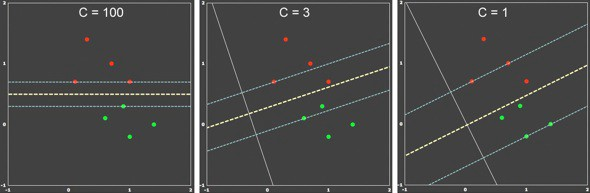
\includegraphics[scale=0.8]{./img/param_c.png}
            \captionsource{Zależność marginesu od parametru C}{\url{https://medium.com/@pushkarmandot}}
            \label{fig:param_c}
        \end{center}
    \end{figure}

    \par Dobry model dobrze separuję dane i razem z tym ma duży margines. Natomiast w
    w rzeczywistości jedno wyłącza drugie: duży margines włącza punkty z dwóch klas, a
    dobre separowanie może powodować przeuczanie(ang. Overfitting). Przeuczanie może 
    skutkować tym że model jest dobry na danych treningowych ale jest zły na danych testowych.

\newpage % description and equations was on different pages
\subsection{$\nu$-SVM}
    \par $\nu$-Support Vector Classification - rodzaj klasyfikatora używający $\nu$ jako
    parametr regularyzacji. Jest bardzo podobny do C-SVM, z różnicą że $\nu\in[0,1]$.
    Przyjemną właściwością $\nu$ jest to że on jest dolną granicą stosunku wektorów
    wspierających i górną granicą stosunku błędu uczenia.
    \par Jeśli jest dany wektor $x_i \in R^n$, $i=1,...,l$ w dwóch klasach i wektor
    $y\in R^l$ taki że $y_i \in \{1, -1\}$ to pierwotny problem optymalizacji wygląda
    następująco:

    \begin{center}
        \begin{tabular}{rl}
            $\min\limits_{\pmb{\omega},b,\varepsilon, \rho}$ &
            $\frac{1}{2}\pmb{\omega}^T\pmb{\omega} - \nu\rho + \frac{1}{l}\sum\limits_{i=1}^{l}
            \varepsilon_i$ \\
            Z zastrzeżeniem że & $y_i(\pmb{\omega}^T\phi(x_i) + b) \geq \rho - \varepsilon_i$ \\
                               & $\varepsilon_i \geq 0$, $i=1,...,l$, $\rho \geq 0$
        \end{tabular}
    \end{center}

\subsection{One-class SVM}
    \par One-class Support Vector Machine - rodzaj klasyfikatora uczenia
    nienadzorowanego, które zakłada brak etykiet w danych uczących. Ma na celu
    znalezienie niewiadomych wzorców/anomalii(klastrów) w danych wejściowych.  

    \begin{figure}[H]
        \begin{center}
            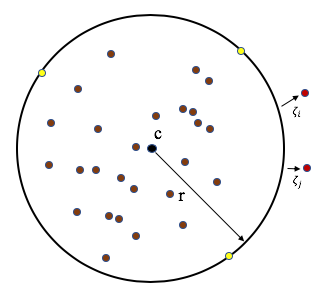
\includegraphics[scale=0.4]{./img/one-class-circle.png}
            \captionsource{Hipersfera zawierająca punkty danych. Ma środek c i promień R.
            Punkty na krawędzi są wektorami wspierającymi.}{Wikipedia. \url{https://en.wikipedia.org/wiki/One-class_classification}}
            \label{fig:one_class}
        \end{center}
    \end{figure}

    \par Jeśli dany jest wektor $x_i\in R^n$, $i=1,...,l$ bez informacji o klasach,
    to pierwotny problem optymalizacji wygląda następująco:

    \begin{center}
        \begin{tabular}{rl}
            $\min\limits_{\pmb{\omega},\varepsilon,\rho}$ & $\frac{1}{2}\pmb{\omega}^T\pmb{\omega} -
            \rho + \frac{1}{\nu l}\sum\limits_{i=1}^{l}\varepsilon_i$ \\
            Z zastrzeżeniem że & $\pmb{\omega}^T\phi(x_i)\geq\rho - \varepsilon_i$,\\
                               & $\varepsilon \geq 0$, $i=1,...,l$
        \end{tabular}
    \end{center}

\newpage
\subsection{$\epsilon$-SVR}
    \par Jeśli wektor etykiet $y_i \in R$ to jest używana metoda regresji.
    $\epsilon$-Support Vector Classification -  używa $C$ i $\epsilon$ jako
    parametrów regularyzacji. Celem jest znalezienie takiej funkcji $f(x)$
    że jej wartość odchyla się od $y_n$ na wartość nie większą od $\epsilon$
    dla każdego punktu z zbioru treningowego.
    \par Jeśli jest dany zbiór danych treningowych $\{(x_1, x_1),...,
    (x_l, z_l)\}$, gdzie $x-I \in R^n$ jest wektorem cech, a $z_i \in R^1$
    jest wyjściem. Przy danych parametrach $C>0$ i $\epsilon > 0$, standardowa 
    forma SVR to:

    \begin{center}
        \begin{tabular}{rl}
            $\min\limits_{\pmb{\omega},b,\pmb{\varepsilon}, \pmb{\varepsilon}^*}$ &
            $\frac{1}{2}\pmb{\omega}^T\pmb{\omega} + C\sum\limits_{i=1}^{l}
            \varepsilon_i + C\sum\limits_{i=1}^{l}\varepsilon_{i}^{*}$ \\
            Z zastrzeżeniem że & $\pmb{\omega}^T\phi(x_i) + b - z_i \leq \epsilon + \varepsilon_i$, \\
                           & $z_i - \pmb{\omega}^T\phi(x_i) - b \leq  \epsilon + \varepsilon_i^*$, \\
                           & $\varepsilon_i,\varepsilon_i^* \geq 0$,$i=1,...,l$

        \end{tabular}
    \end{center}

\subsection{$\nu$-SVR}
    \par $\nu$-Support Vector Regression - podobnie do $\nu$-SVC, używa parameter $\nu\in(0,1]$
    dla kontroli liczby wektorów wspierających. Również używa parametru $\epsilon$. Z parametrami
    $(C,\nu)$ $\nu$-SVR rozwiązuję:
    
    \begin{center}
        \begin{tabular}{rl}
            $\min\limits_{\pmb{\omega},b,\pmb{\epsilon},\pmb{\epsilon}^*,\epsilon}$ &
            $\frac{1}{2}\pmb{\omega}^T\pmb{\omega} + C(\nu\epsilon + \frac{1}{l}
            \sum\limits_{i=1}^{l}(\varepsilon_i+\varepsilon_i^*))$ \\
            Z zastrzeżeniem że & 
            $(\pmb{\omega}^T\phi(x_i) + b) - z_i \leq \epsilon + \varepsilon_i$,\\
           & $z_i - (\pmb{\omega}^T\phi(x_i) + b) \leq \epsilon + \varepsilon_i^*$,\\
           & $\varepsilon_i,\varepsilon_i^* \geq 0$, $i=1,...,l$, $\epsilon \geq 0$
        \end{tabular}
    \end{center}

\subsection{Jądra}
    \par W przypadku kiedy klasy nierozdzielne liniowo to jest używany trik z zastosowaniem
    funkcji jądrowych(ang. Kernel Trick). Funkcję jądrowe pozwalają odwzorować zbiór danych
    w przestrzeń z większą liczbą wymiarów, w której klasy danego zbioru będzie można rozdzielić
    hiperpłaszczyzną. 

    \begin{figure}[H]
        \begin{center}
            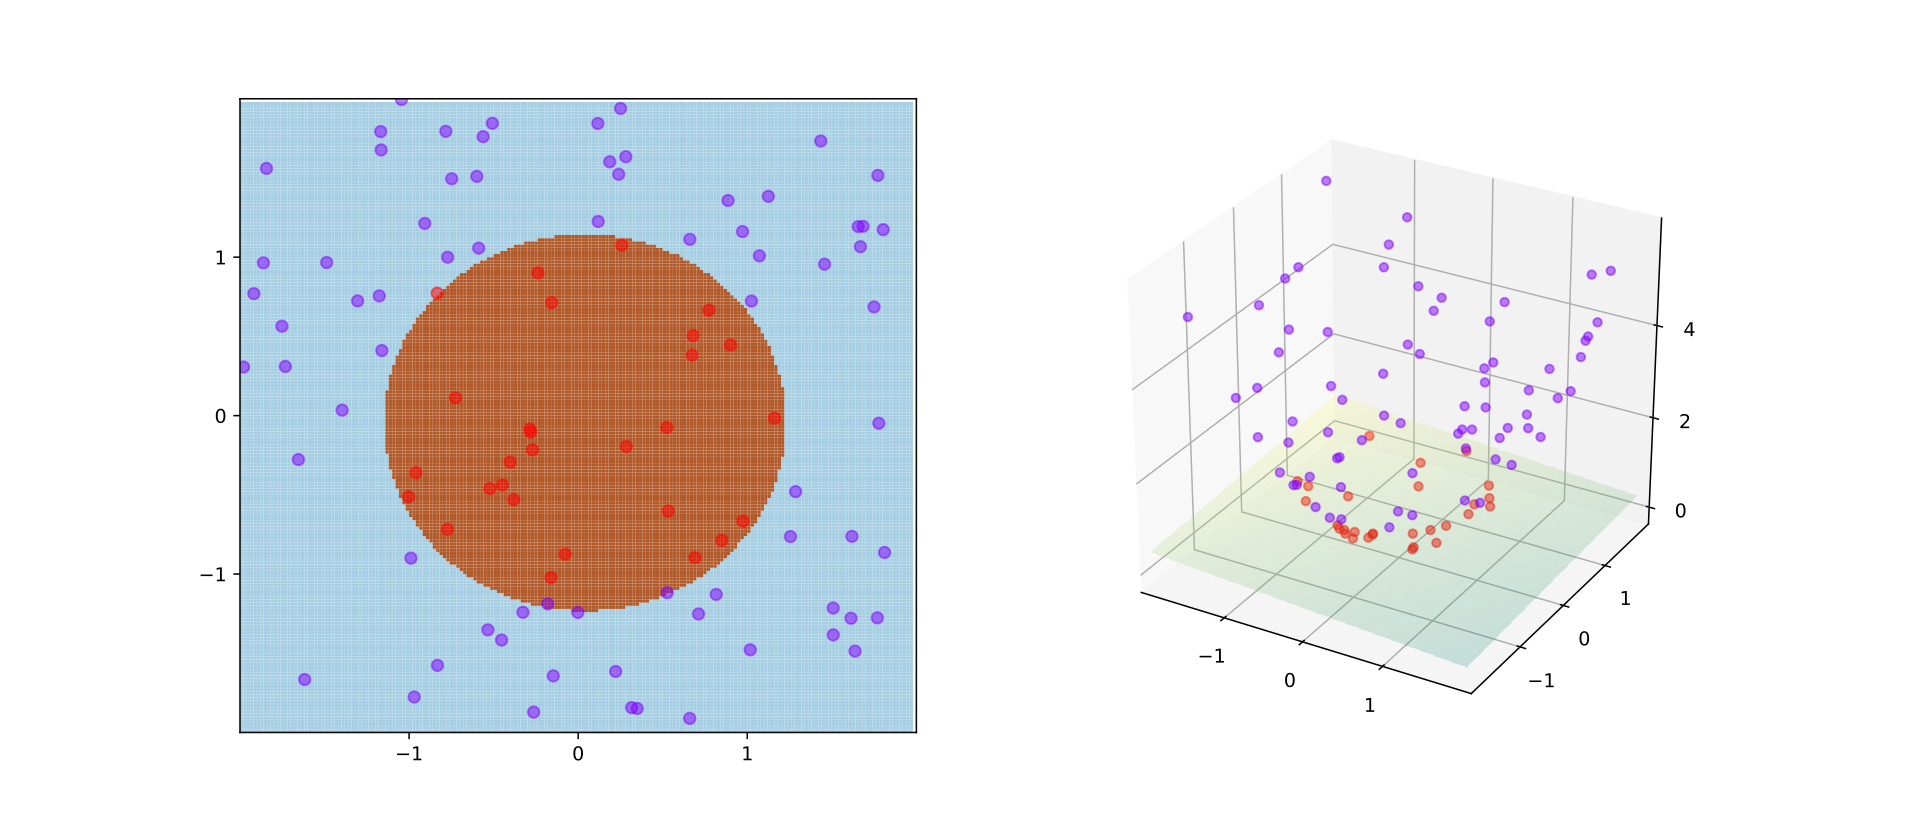
\includegraphics[scale=0.2]{./img/kernel_trick.png}
        \captionsource{Przykład stosowania funkcji jądrowej dla nierozdzielnego liniowo zbioru
        danych}{Wikipedia. \url{https://en.wikipedia.org/wiki/Kernel_method}}
        \label{fig:kernel_trick}
        \end{center}
    \end{figure}

    \newpage 

    \par W bibliotece LIBSVM są zaimplementowane następne funkcje jądrowe:

    \begin{center}
        \begin{tabular}{rl}
            Liniowa & $K(x,x') = x\cdot x'$\\
            Wielomianowa & $K(x,x') = (\gamma*x \cdot x'+coef0)^{degree})$\\
            RBF & $K(x,x') =  -\gamma * (\sqrt{x}+\sqrt{x'}-2 * x\cdot x')$ \\
            Sigmoidalna & $K(x,x') = tanh(\gamma*x \cdot x'+coef0)$
        \end{tabular}
    \end{center}

    \par Autorzy biblioteki LIBSVM polecają \cite{hsu2003practical} że pierwsza funkcja jądrowa
    którą warto spróbować to RBF.  Jak pokazują \cite{keerthi2003asymptotic} jeśli używać RBF z
    optymalizacją hiperparametrów to nie ma potrzeby rozważać liniową funkcję jądrową. W sigmoidalnej
    funkcji jądrowej macierz jądrowa może nie być pozytywnie określona i generalnie dokładność modelu
    nie jest lepsza od RBF \cite{lin2003study}. 

\newpage
\section{Wymagania} % SECTION
\subsection{Wymagania ogólne}
    \par Aplikacja ma implementować uczenie maszynowe metodą SVM. Uczenie ma być dwufazowe:
    trenowanie i testowanie. Pod czas trenowania aplikacja ma generować model w postaci pliku.
    Na etapie testowania aplikacja ma mieć możliwość załadowania dowolnego pliku z modelem.

\subsection{Sterowanie aplikacją \textbf{\textcolor{red}{LEPSZA NAZWA?}}} % TODO: remove
    \par Sterowanie aplikacją musi odbywać się wyłącznie przez Interfejs graficzny. Interfejs
    graficzny użytkownika ma być zorganizowany w sposób podkreślający to że nauczanie jest
    dwufazowe. Akcje które użytkownik nie może zrobić przez ich bezsensowność lub
    niedostępność na danym etapie muszą być zablokowane w sposób oczywisty dla użytkownika.

\subsection{Wejście/Wyjście}
    \par Program na wejściu otrzymuje co najmniej jeden plik z danymi zawierający cechy i
    etykiety. Wyjściem jest plik z modelem i wypisywana na interfejsie graficznym precyzja
    modelu w przypadku testowania. 

\subsection{Wizualizacja}
    \par Aplikacja musi umieć wizualizować dane wejściowe jedno, dwu i trzy wymiarowe. Dla
    jedno i dwu wymiarowych danych program musi mieć możliwość generowania wykresu gęstości
    rozkładu. Dla celów dydaktycznych aplikacja musi umieć wizualizować wytrenowany model.

\subsection{Przypadki użycia}
\subsubsection{Przypadek użycia 1. Trenowanie modelu}

\begin{tabular}{|l|l|}  \hline
    \textbf{Nazwa} & Wytrenuj model \\\hline
    \textbf{Inicjator} & Użytkownik \\\hline
    \textbf{Cel} & Wygenerowanie pliku modelu \\\hline
    \textbf{Warunki wstępne} & brak\\\hline
    \textbf{Główny scenariusz} & 
    \begin{minipage}{5in}
        \vskip 4pt
        \begin{enumerate}
            \item Użytkownik ładuje plik z danymi do trenowania do aplikacji.
            \item Aplikacja sprawdza czy format danych jest poprawny.
            \item Użytkownik wprowadza odpowiednie parametry modelu.
            \item Użytkownik uruchamia trenowanie.
            \item Aplikacja generuje trenuje model i zapisuje do pliku.
        \end{enumerate}
        \vskip 4pt
    \end{minipage}
    \\\hline

    \textbf{Rozszerzenia} & 
    \begin{minipage}{5in}
        \vskip 4pt
        \begin{itemize}
            \item[2a.] Wgrany zbiór danych nie jest w formacie \textit{LIBSVM}.
                \begin{itemize}
                    \item[a.] Użytkownik konwertuje swój zbiór danych do formatu \textit{LIBSVM}.
                    \item[c.] Użytkownik kontynuuje scenariusz główny z p.3.
                \end{itemize}
            \item[3a.] Użytkownik wprowadził tekstowy symbol w pole z liczbami.
                \begin{itemize}
                    \item[a.] Aplikacja podświetla niepoprawny parametr na czerwono.
                    \item[b.] Użytkownik robi korektę błędnego parametru.
                    \item[c.] Użytkownik kontynuuje scenariusz główny z p.4.
                \end{itemize}
        \end{itemize}
        \vskip 4pt
    \end{minipage}
    \\\hline
\end{tabular}

\subsubsection{Przypadek użycia 2. Testowanie modelu}
\begin{tabular}{|l|l|}  \hline
    \textbf{Nazwa} & Testuj model \\\hline
    \textbf{Inicjator} & Użytkownik \\\hline
    \textbf{Cel} & Otrzymać informacje o precyzji modelu \\\hline
    \textbf{Warunki wstępne} & Użytkownik wytrenował model.\\\hline
    \textbf{Główny scenariusz} & 
    \begin{minipage}{5in}
        \vskip 4pt
        \begin{enumerate}
            \item Użytkownik ładuje plik z testującym zbiorem danych do aplikacji.
            \item Użytkownik wprowadza procent walidacji(ile rekordów z zbioru trenującego
                wybrać do testowania)
            \item Użytkownik uruchamia testowanie.
            \item Aplikacja przeprowadza testowanie i walidacje modelu.
            \item Aplikacja wypisuje wyniki testowania i walidacji w polu tekstowym.
        \end{enumerate}
        \vskip 4pt
    \end{minipage}
    \\\hline

    \textbf{Rozszerzenia} & 
    \begin{minipage}{5in}
        \vskip 4pt
        \begin{itemize}
            \item[2a.] Załadowany plik jest niepoprawny(inna liczba cech/klas niż w pliku
                trenującym)
                \begin{itemize}
                    \item[a.] Aplikacja podświetla ścieżkę do pliku na czerwono.
                    \item[b.] Użytkownik ładuje poprawny plik.
                    \item[c.] Użytkownik kontynuuje główny scenariusz z p.3.
                \end{itemize}
        \end{itemize}
        \vskip 4pt
    \end{minipage}
    \\\hline
\end{tabular}

\subsubsection{Przypadek użycia 3. Wizualizacja danych}
\begin{tabular}{|l|l|}  \hline
    \textbf{Nazwa} & Wizualizuj dane \\\hline
    \textbf{Inicjator} & Użytkownik \\\hline
    \textbf{Cel} & Przedstawić dane w postaci graficznej \\\hline
    \textbf{Warunki wstępne} & Użytkownik załadował plik z danymi do trenowania\\\hline
    \textbf{Główny scenariusz} & 
    \begin{minipage}{5in}
        \vskip 4pt
        \begin{enumerate}
            \item Użytkownik uruchamia wizualizacje danych.
            \item Aplikacja wczytuje dane z pliku trenującego.
            \item Aplikacja rysuje punkty na płaszczyźnie w nowym oknie.
        \end{enumerate}
        \vskip 4pt
    \end{minipage}
    \\\hline

    \textbf{Rozszerzenia} & 
    \begin{minipage}{5in}
        \vskip 4pt
        \begin{itemize}
            \item[1a.] Przycisk wizualizacji jest nieaktywny.
                \begin{itemize}
                    \item[a.] Użytkownik sprawdza liczbę cech w podanym pliku trenującym.
                    \item[b.] Użytkownik ładuje plik z danymi, w którym liczba cech jest
                        mniejsza lub równa 3.
                    \item[c.] Użytkownik kontynuuje główny scenariusz z p.1.
                \end{itemize}
        \end{itemize}
        \vskip 4pt
    \end{minipage}
    \\\hline
\end{tabular}

\subsection{Obsługa błędów}
    \par Informacja o błędach występujących w trakcie działania aplikacji będzie przekazywana
    do użytkownika w polu tekstowym lub w postaci podświetlenia na czerwono elementu interfejsu
    w którym jest błąd. 
    \par Informacja o błędach wewnętrznych(Maszyna wirtualna Python, system operacyjny zamknął
    aplikacje z powodu naruszenia ochrony pamięci) będą od użytkownika ukryte. Zaawansowane
    użytkowniki będą mogli uruchomić aplikacje z konsoli, w której takie błędy będą wypisywane,
    by naprawić środowisko w którym uruchamiają aplikacje.

\subsection{Środowisko wywołania}
    \par Aplikacja jest tworzona dla systemu operacyjnego Linux. Użytkownicy systemu operacyjnego
    OS X(wcześniej macOS) będą mogli skompilować i uruchomić aplikacje po instalacji wszystkich
    zależności. Kompilacja i uruchomienie aplikacji na systemie operacyjnym Windows nie są
    wspierane, chociaż może to być możliwe, ze względu na to, że użyte technologie są
    wieloplatformowe(ang. cross platform).

\newpage
\section{Analiza wymagań} %SECTION
\subsection{Języki programowania}
    \par Dla napisania aplikacji wybrałem język programowania \textit{C++}. Wybrałem ten język
    programowania przez jego wydajność mimo to że jest on językiem wysokiego poziomu. Na wybór
    \textit{C++} również wpłynęła moja sympatia do tego języka programowania, a napisanie
    dużego projektu w nim było dla mnie prawdziwym wyzwaniem, które pozwoliło pogłębić swoją
    wiedze w programowaniu i używaniu języka \textit{C++}. 

    \par Dla niektórych części programu będzie użyty język \textit{Python}, w szczególności dla
    tych, które dotyczą rysowania wykresów, pracy z plikami i zmiennymi typu \textit{string}.
    Standardowa biblioteka Python przedstawia sporo narzędzi dla pracy z plikami i zmiennymi
    typu \textit{string}, co pozwala oszczędzać czas programisty w porównaniu do C++, w którym
    napisanie podobnej funkcjonalności zajęłoby o wiele więcej czasu. 

\subsection{Rysowanie wykresów}
    \par Dla rysowania wykresów wybrałem bibliotekę \textit{matplotlib} \cite{matplotlib} która
    pozwala stosunkowo łatwo rysować jedno, dwu i trzy-wymiarowe wykresy, a w kombinacji z
    \textit{numpy} i \textit{scipy} generować wykresy gęstości.  

\subsection{Interfejs graficzny}
    \par Dla implementacji interfejsu graficznego wybrałem wieloplatformową bibliotekę
    \textit{Qt} \cite{qtlibrary} napisanej w C++.  Twórcy biblioteki \textit{Qt} stworzyli IDE
    dedykowane do pracy z biblioteką - \textit{Qt Creator}. Jest ono wyposażone w szczegółową
    dokumentacje do biblioteki, wbudowany program \textit{Qt Designer} pozwala projektować
    interfejs graficzny metodą przeciągnij i upuść(ang. drag and drop), automatyczne
    uzupełnienie kodu, prowadzi analizę semantyczną kodu i wskazuje na błędy jeszcze przed
    kompilacją.

\subsection{Biblioteki implementujące metodę uczenia SVM}
    \par Istnieje mnóstwo implementacji metody uczenia SVM. Autorzy strony \textit{SVM -
    Support Vector Machines}\cite{svm_soft} zebrali listę oprogramowania implementującego
    metodę uczenia SVM. Z tej listy, ze względu na to żę jako główny język programowania dla
    swojej aplikacji wybrałem \textit{C++}, pasowali mi tylko te biblioteki: \textit{SVMLight},
    \textit{mySVM}, \textit{LIBSVM}, \textit{SVMTorch}. 

    \par Przewagę oddałem \textit{LIBSVM} z uwagi na dobrą dokumentację, obecność instrukcji
    dla nowicjuszy i dobry rozdział FAQ, który wytłumaczył mi wiele pytań o działaniu tej
    biblioteki.

\subsection{\textit{LIBSVM}} 
    \par \textit{LIBSVM} napisana w 2011 roku przez Chih-Chung Chang i Chih-Jen Lin w
    Państwowym Uniwersytecie Tajwańskim. Celem autorów było zrobienie narzędzia z prostym
    interfejsem umożliwiające używanie Maszyny Wektorów Wspierajacych użytkownikom które nie
    zajmują się zawodowo nauczaniem maszynowym. Domyślnie użycie biblioteki \textit{LIBSVM}
    polega na skompilowaniu i używaniu dwóch programów: \textit{svm-train} i
    \textit{svm-predict}. \textit{svm-train} służy do trenowania modelu, a \textit{svm-predict}
    do testowania, chociaż również może być używany do klasyfikacji nowych niegrupowanych
    danych. 

    \begin{figure}[H]
        \begin{center}
            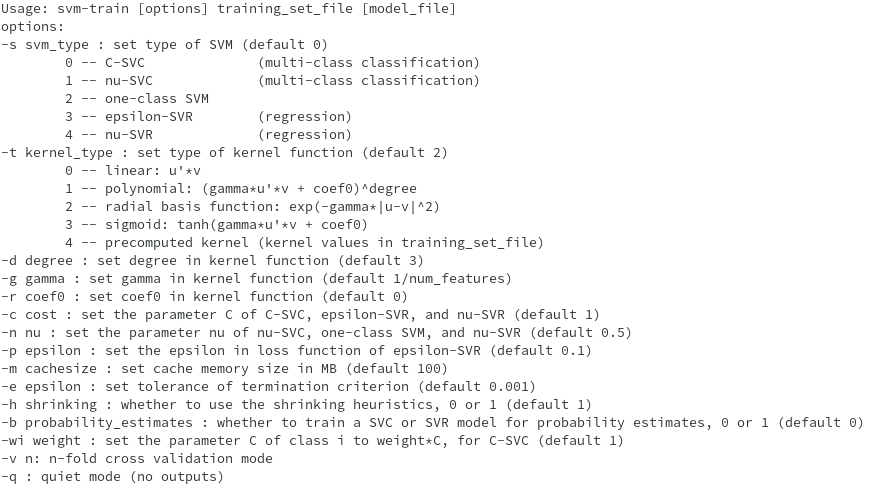
\includegraphics[scale=0.6]{./img/svm_train_usage.png}
            \caption{Użycie programu svm-train}
            \label{fig:train_usage}
        \end{center}
    \end{figure}

    \begin{figure}[H]
        \begin{center}
            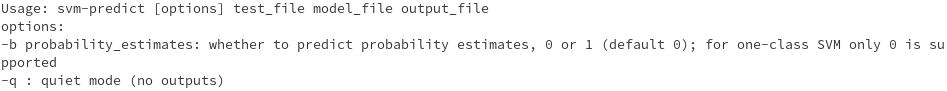
\includegraphics[scale=0.6]{./img/svm_predict_usage.png}
            \caption{Użycie programu svm-predict}
            \label{fig:predict_usage}
        \end{center}
    \end{figure}

\newpage 
\section{Projekt} % SECTION
\subsection{Model danych}
    \par \textit{LIBSVM} domyślnie używa tak zwany "rzadki" format danych z etykietowanymi
    wektorami. Format danych do trenowania i testowania jest taki:

    \begin{verbatim}
    <label> <index1>:<value1> <index2>:<value2> ...
    .
    .
    .
    \end{verbatim}

    \par Każda linia jest osobną instancją i kończy się znakiem '\textbackslash n'.
    Etykiety(ang. label) są używane na różne sposoby: \cite{CC01a}
    \begin{itemize}
        \item Dla klasyfikacji: etykieta jest liczbą naturalną określającą klasę.
        \item Dla regresji: etykieta jest wartością docelową i może być dowolną liczbą
            rzeczywistą.
        \item Dla jednoklasowego SVM(ang. one-class SVM) etykiety nie są używane i mogą być
            dowolne.
    \end{itemize}

    Jeśli w danym wektorze wartość cechy jest 0 to można ją pominąć, np. wektor $[1, 0, 3, 0]$
    w formacie \textit{LIBSVM} można zapisać tak:
    \begin{verbatim}
    1:1 3:3
    \end{verbatim}

    Aplikacja zachowuję intencję twórców biblioteki \textit{LIBSVM}: rozdzielić uczenie na fazy
    trenowania i testowania, a więc użycia dwóch plików z danymi. Pliki trnujące i testujące są
    zapisywane w takim samym formacie i różnią się tylko celem do którego będą użyte.

    \subsection{Szkielet kodu}
    \par W projekcie aplikacji starałem się napisać kod w kształcie modułów, każdy z których
    odpowiada za swoją część funkcjonalności.

    \subsubsection{Sygnały i gniazda Qt}
    \par Mechanizm sygnałów i gniazd biblioteki \textit{Qt} \cite{qtsignalslot} jest powszechnie używany w projekcie
    aplikacji. Sygnały najczęściej są wywoływane przez kontrolki na interfejsie graficznym, a
    gniazdem jest funkcja do której są przekazywane odpowiednie parametry. Na przykład sygnał
    \textit{AvailabilityHandler::testEnabled} odpowiadający za dostępność testowania modelu
    jest połączany z czterema gniazdami: 
    \newpage
    \begin{lstlisting}
connect(availability_handler, &AvailabilityHandler::testEnabled, ui(*@-@*)>test_pushButton, &QPushButton::setEnabled);
connect(availability_handler, &AvailabilityHandler::testEnabled, ui(*@-@*)>validation_label, &QLabel::setEnabled);
connect(availability_handler, &AvailabilityHandler::testEnabled, ui(*@-@*)>validation_percent_label, &QLabel::setEnabled);
connect(availability_handler, &AvailabilityHandler::testEnabled, ui(*@-@*)>validation_lineEdit, &QLineEdit::setEnabled);
    \end{lstlisting}

    \par Co pozwala za pomocą wywołania jednej funkcji
    \textit{AvailabilityHandler::testEnabled} deaktywować cztery elementy interfejsu.

    \begin{figure}[H]
        \begin{center}
            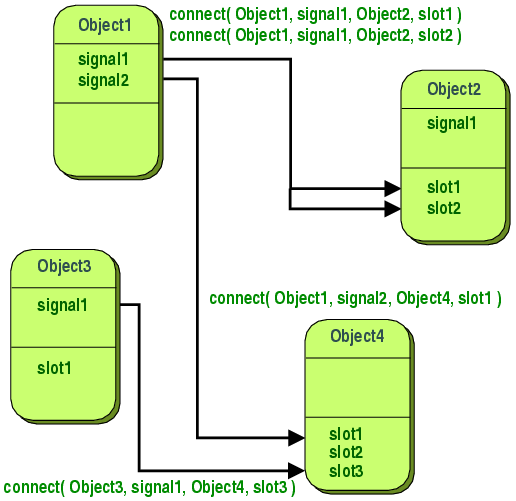
\includegraphics[scale=0.6]{./img/signal_slots.png}
            \caption{Wizualizacja systemu sygnałów i
            gniazd \cite{qtsignalslot}}
            \label{fig:signal_slots}
        \end{center}
    \end{figure}

\newpage 

    \par Przykład kodu w którym sygnały wywoływane w klasie \textit{AvailabilityHandler} są łączone
    z gniazdami w kontrolkach z polami do wpisywania parametrów.

    \begin{lstlisting}
connect(availability_handler, &AvailabilityHandler::degreeEnabled, ui(*@-@*)>degree_spinBox, &QSpinBox::setEnabled);
connect(availability_handler, &AvailabilityHandler::gammaEnabled, ui(*@-@*)>gamma_lineEdit, &QLineEdit::setEnabled);
connect(availability_handler, &AvailabilityHandler::coef0Enabled, ui(*@-@*)>coef0_lineEdit, &QLineEdit::setEnabled);
connect(availability_handler, &AvailabilityHandler::cEnabled, ui(*@-@*)>C_lineEdit, &QLineEdit::setEnabled);
connect(availability_handler, &AvailabilityHandler::nuEnabled, ui(*@-@*)>nu_lineEdit, &QLineEdit::setEnabled);
connect(availability_handler, &AvailabilityHandler::pEnabled, ui(*@-@*)>P_lineEdit, &QLineEdit::setEnabled);
    \end{lstlisting}

    \par Żeby wyżej wymienione sygnały wywoływały się automatycznie sygnały kontrolek
    \textit{Combo Box} zmieniających typ SVM lub funkcje jądrową są łączone z gniazdami w
    klasie \textit{AvailabilityHandler}:

    \begin{lstlisting}
connect(ui->svmType_comboBox, SIGNAL(currentIndexChanged(int)), availability_handler, SLOT(filterSVMTypeParams(int)));
connect(ui->kernel_comboBox, SIGNAL(currentIndexChanged(int)), availability_handler,SLOT(filterKernelParams(int)));
    \end{lstlisting}

    \par Z sygnału \textit{currentIndexChanged} jest przekazywany indeks wybranego elementu do
    gniazda \textit{filterSVMTypeParams} w którym są wywoływany odpowiednie sygnały
    zarządzające dostępnością parametrów.

    \newpage
    \subsubsection{Klasy C++}
    Krótkie opisy najważniejszych klas:\\

    \begingroup
    \setlength{\tabcolsep}{10pt} % Default value: 6pt
    \renewcommand{\arraystretch}{1.5}
    \begin{tabular}{p{0.2\textwidth}p{0.7\textwidth}} % \hline
        \textbf{Nazwa klasy} & \textbf{Opis funkcjonalności} \\ % \hline
        AvailabilityHandler &  
        Klasa sterująca dostępnością elementów interfejsu użytkownika. Używa mechanizmu
        sygnałów i gniazd biblioteki \textit{Qt}, co pozwala na to, żeby wywołanie metody np.
        \textit{trainButtonEnabled} powodowało zmianę stanu na interfejsie graficznym. 
        \\ % \hline
        FileManager & 
        Klasa zarządza ładowaniem plików do aplikacji, odświeżaniem ścieżek plików i informacji
        o pliku(takich jak liczba cech, rekordów i klas).
        \\ % \hline
        OutputHandler &
        Klasa odpowiada za wypisywanie tekstu w polu tekstowym. Tworzy potok do którego
        przekierowuje \textit{stdout} i uruchamia wątek który czyta z potoku i wszystko co
        przychodzi na standardowe wyjście wypisuje do interfejsu użytkownika.
        \\ % \hline
        ScriptQtManager & 
        Klasa odpowiada za uruchamianie skryptów w języku \textit{Python}. Przekazuje
        właściwe parametry do skryptów i zwraca wyjście skryptu do kodu w C++.
        \\ % \hline
        SVMController &
        Klasa pomaga zminimalizować użycie polecenia \textit{system()}(uruchamia komendę z
        powłoki sh). Faktycznie klasa opakowuje funkcje biblioteki \textit{LIBSVM}, żeby
        wygodnie ich można było używać z kodu C++.
        \\ % \hline
        svmscale &
        Klasa opakowuje funkcjonalność programu \textit{svm-scale} dostarczanego z biblioteką
        \textit{LIBSVM}, pozwala zminimalizować użycie polecenia \textit{system()} i uruchamiać
        skalowanie danych bezpośrednio z kodu C++.
        \\ % \hline
        MainWindow & 
        Jest jądrem aplikacji, ustawia wszystkie sygnały. Reakcje na kliknięcia w przyciski są
        zdefiniowane w tej klasie. 
        \\ % \hline
    \end{tabular}
    \endgroup

    \newpage
\subsubsection{Skrypty Python}
    Krótkie opisy skryptów w języku \textit{Python}: \\

    \begingroup
    \setlength{\tabcolsep}{10pt} % Default value: 6pt
    \renewcommand{\arraystretch}{1.5}
    \begin{tabular}{p{0.2\textwidth}p{0.7\textwidth}} % \hline
        \textbf{Nazwa pliku} & \textbf{Opis funkcjonalności} \\ % \hline
        checkdata.py & 
        Skrypt dostarczany z biblioteką \textit{LIBSVM}, sprawdza czy dane w pliku mają format
        \textit{LIBSVM}. Na podstawie wyniku działania tego skryptu aplikacja decyduje czy plik
        z danymi może być użyty do trenowania lub testowania.
        \\ % \hline
        convert2svm.py &
        Skrypt który stara się skonwertować plik z danymi do formatu \textit{LIBSVM}. Na
        wejściu wymaga podania ścieżki do pliku z danymi w formacie innym niż \textit{LIBSVM},
        nazwa pliku wyjściowego z danymi w formacie \textit{LIBSVM}, separator cech, separator
        dziesiętny(przecinek lub kropka) i ostatni parametr 1 - jeśli etykieta jest na początku
        linii i 0 - na końcu linii. Plik wynikowy jest sprawdzany skryptem
        \textit{checkdata.py} żeby zapobiec trenowaniu przy pomocy błędnego pliku który może
        powstać przez błąd użytkownika(np. podanie niepoprawnego separatora cech).
        \\ % \hline
        f\_select.py &
        Skrypt pozwala wybrać które cechy są potrzebne w procesie nauczania modelu. Na wejściu
        wymaga podania pliku z danymi, liczbę cech i jakie cechy należy wybrać. Wyjściem
        skryptu jest plik z danymi z rozszerzeniem \textit{.fselected}.
        \\ % \hline
        grid.py & 
        Skrypt dostarczany z biblioteką \textit{LIBSVM} służy do dobierania najlepszych
        parametrów dla trenowania modelu. Na wejściu wymaga podania początkowych i końcowych
        wartości dla poszczególnych parametrów oraz krok z którym algorytm "idzie" parametrem.
        \\ % \hline
        h4c.py i h4r.py &
        Holdout dla klasyfikacji i holdout dla regresji. Skrypty pozwalające na podział jednego
        pliku z danymi na zbiory trenujący i testujący. Skrypty wymagają na wejściu ścieżkę do
        pliku z danymi oraz procent danych który ma być wybrany dla testowania. \textit{h4c.py}
        stara się zachować stosunek klas w zbiorze testującym taki sam jak w pierwotnym pliku,
        a \textit{h4r.py} losowo wybiera wskazany procent rekordów. \textit{h4r.py} jest
        również używany do walidacji.
        \\ % \hline 
        plotter.py & 
        Skrypt służy do wizualizacji danych za pomocą biblioteki \textit{matplotlib}. Umie
        rysować jedno- dwu- i trzy-wymiarowe wykresy, dla jednego i dwóch wymiarów są również
        dostępne wykresy gęstości.
        \\ % \hline
        pointsgen.py & 
        Skrypt pozwala użytkownikom na ręczne generowanie danych. Po uruchamianiu skryptu
        otwiera się okno w którym są rejestrowane kliknięcia myszą i na ich miejscu są rysowane
        punkty. Po zamknięciu okna jest generowany plik z wygenerowanymi danymi.
        \\ % \hline
    \end{tabular}
    \endgroup

\subsection{Organizacja plików}
    \par Kod aplikacji, wszystkie użyte zbiory danych i żródła biblioteki \textit{LIBSVM}
    znajdują się na repozytorium pod adresem \url{https://github.com/boidachenkop/svm-app}.
    Źródła aplikacji znajdują się w katalogu \textit{svm-app}, dla edycji lub przeglądu kodu
    zaleca się używania IDE(od ang. integrated development environment) \textit{Qt Creator}
    \cite{qtcreator}, skoro potrafi ono automatycznie posortować pliki .cpp, .h, .py oraz
    przedstawić schemat interfejsu graficznego na podstawie pliku \textit{mainwindow.ui}.
    \par Wszystkie zbiory danych używane dla przykładów znajdują się w katalogu
    \textit{datasets}. Oryginalny kod żródłowy biblioteki \textit{LIBSVM} znajduje się w
    katalogu \textit{libsvm-3.23}.

\newpage
\section{Implementacja} % SECTION

    \par Po uruchomieniu programu pierwsze co zobaczy użytkownik - okno główne. Po lewej
    stronie jest pole tekstowe w którym pojawiają się komunikaty o wynikach trenowania lub
    testowania modelu. W prawej górnej części okna są kontrolki do wybierania plików z danymi
    lub zapisywania pliku modelu. Żeby rozdzielić główną funkcjonalność od pobocznej i zrobić
    okno główne programu bardziej kompaktowym niektóre elementy są zrealizowane w postaci kart,
    natomiast funkcjonalność która dotyczy trenowania i testowania modelu jest
    dostępna bezpośrednio z okna głównego.

    \begin{figure}[H]
        \begin{center}
            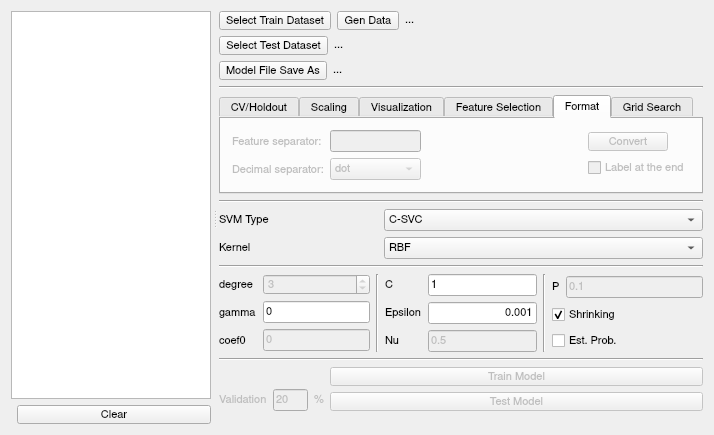
\includegraphics[scale=0.7]{./img/svm_app_main_window.png}
            \caption{Okno główne programu}
            \label{fig:main_window}
        \end{center}
    \end{figure}

\newpage % for better look
\subsection{Pole tekstowe dla komunikatów.}

    \begin{figure}[H]
        \begin{center}
            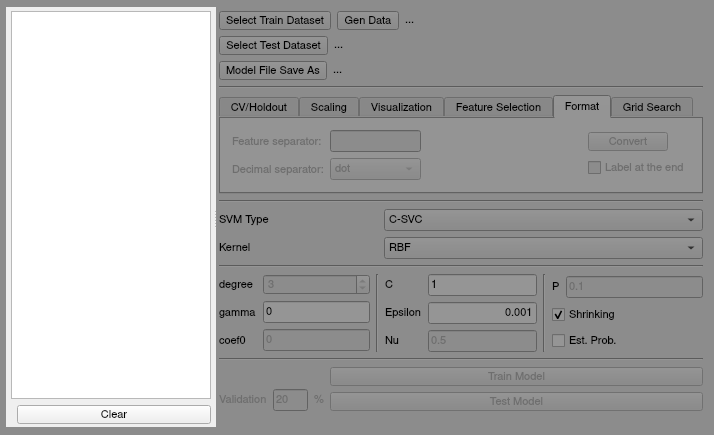
\includegraphics[scale=0.7]{./img/svm_app_mainw_textedit.png}
            \caption{Pole dla komunikatów}
            \label{fig:text_edit}
        \end{center}
    \end{figure}

    \par Pole tekstowe \ref{fig:text_edit} w lewej części okna głównego programu przyznaczone
    dla wypisywania komunikatów z biblioteki \textit{LIBSVM} lub używanych skryptów Python. W
    zasadzie opisywana kontrolka jest widżetem biblioteki \textit{Qt} \textit{TextEdit} w
    którym jest wyłączona możliwość edytowania zawartości. Dla tego żeby nie przerabiać kodu
    żródłowego biblioteki \textit{LIBSVM} zamieniając każde wywołanie funkcji \textit{printf}
    na odpowiednią funkcje, któraby dodawała tekst na \textit{TextEdit}, szukałem sposobu na
    przekierowanie całego wyjścia aplikacji na widżet w interfejsie graficznym. Niestety
    biblioteka \textit{Qt} nie przedstawia prostej możliwości na zrobienie tego, więc musiałem
    zraimplementować podobną funkcjonalność samodzielnie. Za tą funkcjonalność odpowiada klasa
    \textit{OutputHandler}, która w swoim konstruktorze tworzy potok do którego przekierowuje
    \textit{stdout}.

    \begin{lstlisting}[caption={Konstruktor klasy \textit{OutputHandler}},captionpos=b]
    OutputHandler::OutputHandler()
    {
        _saved_stdout = dup(STDOUT_FILENO);
        pipe(_stdout_pipe);
        dup2(_stdout_pipe[1], STDOUT_FILENO);
        close(_stdout_pipe[1]);
    }
    \end{lstlisting}

    \par Za tym uruchamia wątek który ciągle sprawdza czy coś było zapisane do potoku i jeśli
    tak to wywołuje sygnał który dopisuje te dane do \textit{TextEdit} na interfejsie graficznym.

    \newpage
    \begin{lstlisting}[caption={Funkcja uruchamiana w wątku},captionpos=b]
    void OutputHandler::handleOutput()
    {
        int bytes_read;
        char buf[1024];
        while((bytes_read = (int)read(_stdout_pipe[0], buf, sizeof(buf))))
        {
            emit updateOutput(QString::fromLatin1(buf, bytes_read));
            if(_cmd_out)
            {
                write(_saved_stdout, buf, bytes_read);
            }
        }
    }
    \end{lstlisting}

    \par Takie podejście pozwala używać standardowe sposoby na wypisywanie komunikatów i nie
    myśleć o tym czy wypisywany komunikat zostanie wyświetlony na interfejsie użytkownika.
    \par Pod omawianym polem tekstowym znajduje się przycisk \textit{Clean}, który usuwa
    wszystkie wcześniej wypisane komunikaty z pola \textit{TextEdit}. 

\subsection{Zarządzanie plikami z danymi}

    \par Pierwszym krokiem który będzie musiał zrobić użytkownik po uruchamianiu aplikacji -
    wybrać plik z danymi dla trenowania. Dla tego celu na ekranie głównym są odpowiednie
    kontrolki \ref{fig:file_handler} które pozwalają wybrać plik z danymi do trenowania lub
    testowania i wybrać katalog w którym należy zapisać plik z wygenerowanym modelem. Domyślnie
    plik modelu ma nazwę [nazwa pliku z danymi do trenowania + .model]. Przycisk \textit{Gen
    Data} pozwala wygenerować plik z danymi samodzielnie, jego funkcjonalność będzie omówiona
    później.

    \begin{figure}[H]
        \begin{center}
            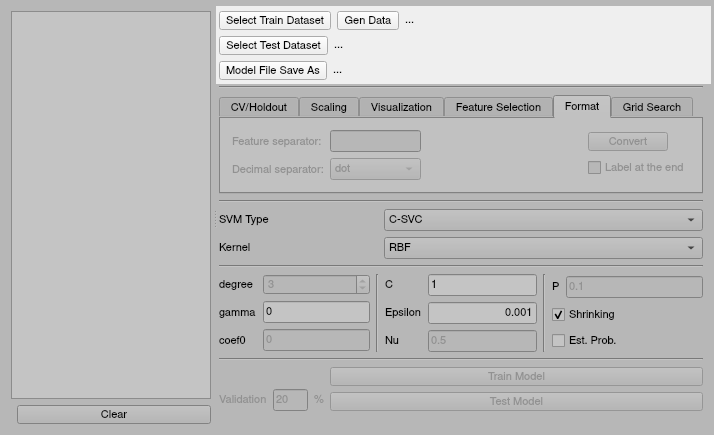
\includegraphics[scale=0.7]{./img/svm_app_mainw_filehandler.png}
            \caption{Zarządzanie plikami}
            \label{fig:file_handler}
        \end{center}
    \end{figure}

    \par Po wybraniu pliku z danymi program sprawdza czy dane są zapisane w formacie
    \textit{LIBSVM}. W przypadku poprawności danych program parsuje plik wypisując liczbę
    rekordów, liczbę klas i liczbę cech jak dla danych trenujących tak i dla danych testowych.

    \begin{figure}[H]
        \begin{center}
            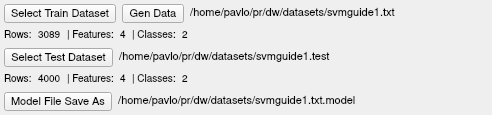
\includegraphics[scale=0.8]{./img/svm_app_mainw_filehandler_ex.png}
            \caption{Przykład wczytanych danych}
            \label{fig:files_example1}
        \end{center}
    \end{figure}

    \par Format danych \textit{LIBSVM} przewiduję klasę na skrajnej lewej pozycji w linii, cechy są
    indeksowane, jeśli cecha równa się 0 to informacja o nich jest zbędna. Warto wspomnieć, że
    wybrana wersja biblioteki \textit{LIBSVM} nie przewiduje użycia danych tekstowych:

    \begin{verbatim}
        1 1:3.5 2:2.25 3:1.17 # komentarz
        -1 2:3  # pierwsza i trzecia cechy są 0
    \end{verbatim}

    \par Poprawność danych wejściowych sprawdza skrypt w języku Python udostępniany w ramach
    biblioteki \textit{LIBSVM}. Jeśli plik mieści niepoprawne dane to ścieżka do wybranego
    pliku jest farbowana na czerwono i jest wypisywany odpowiedni komunikat. W przypadku
    \ref{fig:files_example1} w pliku z danymi linia 19 mieści cechę wartość której ma liczbę
    rzeczywistą z przecinkiem, a w formacie danych \textit{LIBSVM} są dopuszczane tylko kropki.

    \begin{figure}[H]
        \begin{center}
            
\includegraphics[scale=0.8]{./img/svm_app_mainw_filehandler_ex_wrong.png}
            \caption{Przykład wczytanych niepoprawnych danych}
            \label{fig:files_example1}
        \end{center}
    \end{figure}

    \par Jeśli dane do testowania nie zgadzają się z danymi do trenowania(np. liczbą cech lub
    liczbą klas) to zbiór do testowania nie jest akceptowany: 

    \begin{figure}[H]
        \begin{center}
            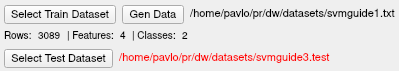
\includegraphics[scale=1.0]{./img/svm_app_mainw_filehandler_ex_wrong2.png}
            \caption{Przykład niezgodności pomiędzy danymi do treningu a danymi do testowania}
            \label{fig:files_example2}
        \end{center}
    \end{figure}

    \par Dzięki bibliotece \textit{Qt}, która w miarę możliwości używa natywnych do systemu
    operacyjnego kontrolek, wygląd selektora plików zależy od systemu operacyjnego. Domyślnie
    selektor plików otwiera katalog \textit{/home/[username]}, ale w przypadku kiedy pliki z
    danymi znajdują się głęboko w systemie plików to może być niewygodne, przez to aplikacja
    przechowuję ostatnio odwiedzony katalog w pliku \textit{/tmp/svmapp-lop} i zawsze otwiera w
    nim nowy selektor plików.

    \par Niektóre akcje użytkownika mogą nie mieć sensu: zacząć proces trenowania bez wybrania
    pliku z danymi, zmieniać parametry modelu które nie dotyczą wybranego typu SVM lub
    wybranej funkcji jądrowej itp. Żeby zapobiec bezsensownym akcjom była zaimplementowana
    klasa \textit{AvailabilityHandler}. Klasa odpowiada za deaktywacje kontrolek funkcjonalność
    których jest bezsensowna lub niebezpieczna \ref{fig:availability_ex} 

    %\newpage % or figure below brakes order

    \begin{figure}[H]
        \begin{subfigure}{.5\textwidth}
            \centering
            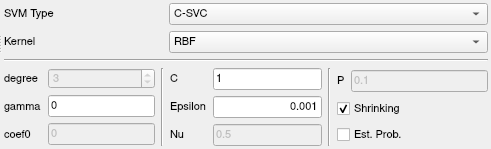
\includegraphics[width=.95\linewidth]{img/svm_app_param_ex1.png}
            \label{fig:availability_ex1}
        \end{subfigure}%
        \begin{subfigure}{.5\textwidth}
            \centering
            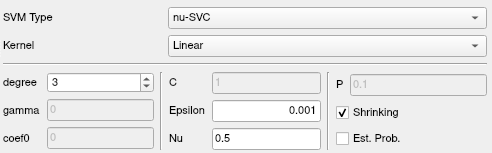
\includegraphics[width=.95\linewidth]{img/svm_app_param_ex2.png}
            \label{fig:availability_ex2}
        \end{subfigure}
        \caption{Przykład zmiany dostępności parametrów w zależności od wybranego typu SVM i
        funkcji jądra}
        \label{fig:availability_ex}
    \end{figure}



\subsection{Parametry SVM i funkcji jądrowych}

    \par Wszystkie parametry oprócz \textit{degree} są w postaci kontrolki \textit{Line Edit} ze
    względu na to że są one liczbami rzeczywistymi, \textit{degree} z kolei jest liczbą
    naturalną a więc używana jest kontrolka \textit{Spin Box}. Po uruchamianiu trenowania
    program czyta pola z parametrami i sprawdza czy są poprawne. W pola typu
    \textit{Line Edit} można wprowadzać litery(ponieważ jest dozwolony zapis liczb w notacji
    naukowej: \textit{1e-3}). Jeśli wprowadzoną liczba nie jest w formacie naukowym lub nie
    jest liczbą rzeczywistą z separatorem kropką, to pole z błędnymi danymi jest obramiane na
    czerwono a proces treningu jest powstrzymywany.

    \begin{figure}[H]
        \begin{center}
            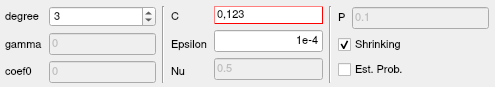
\includegraphics[scale=1.0]{./img/svm_app_param_wrong.png}
            \caption{Przykład niepoprawnych danych w polu parametru C}
            \label{fig:param_wrong}
        \end{center}
    \end{figure}

\subsection{Przyciski trenowania i testowania}


    \par Przyciski trenowania i testowania \ref{fig:train_test_buttons} są umieszczone w dolnej
    części okna głównego programu.

    \begin{figure}[H]
        \begin{center}
            
\includegraphics[scale=1.0]{./img/train_test_buttons.png}
            \caption{Przyciski do trenowania i testowania modelu}
            \label{fig:train_test_buttons}
        \end{center}
    \end{figure}

    \par Po wciśnięciu przycisku \textit{Train Model} aplikacja, jak opisano wyżej,
    parsuje i sprawdza pola z parametrami i uruchamia proces trenowania dokładnie ten który
    oferuję program \textit{svm-train} z biblioteki \textit{LIBSVM}. Żeby ściślej powiązać
    aplikację z biblioteką \textit{LIBSVM} przerobiłem biblioteczne plik źródłowe
    \textit{svm-train.c} i \textit{svm-predict.c} na klasę \textit{SVMController}, pozwoliło to
    zapobiec używaniu polecenia \textit{system()} które służy do uruchamiania programów
    zewnętrznych. Nie udało się jednak całkiem uniknąć tego - skrypty w języku Python używają
    \textit{system()}.

    Przykład wyjścia algorytmu trenującego LIBSVM C-SVC z funkcją jądrową RBF i parametrami
    $C=1$, $gamma=0$:

    \begin{verbatim}
        *
        optimization finished, #iter = 318
        nu = 0.469505
        obj = -383.582676, rho = 0.903354
        nSV = 408, nBSV = 401
        Total nSV = 408
    \end{verbatim}

    \par Gdzie \textit{obj} oznacza wartość optymalną dla problemu podwójnego SVM, \textit{rho}
    jest błędem systematycznym w funkcji decyzyjnej $sgn(w^{T}x - rho)$, \textit{nSV} jest
    liczbą wektorów wspierających, \textit{nBSV} - liczba ograniczonych  wektorów
    wspierających. $\nu$-SVC równoważną formą do C-SVC, nu - jest odpowiednikiem podanego
    parametru C tylko w $\nu$-SVC, czyli jeśli użyć $\nu$-SVC i podać jako parametr $\nu$
    liczbę $0.469505$ to wygenerowany model będzie miał bardzo podobne charakterystyki.

    \par Za przyciskiem \textit{Test Model} poza funkcjonalnością programu \textit{svm-predict}
    stoi jeszcze jedna - walidacja. Klasa \textit{SVMController} wczytuje plik z danymi do
    testowania i wypisuje procent dobrych zgadnięć wygenerowanego modelu, po tym w zależności
    od wartości w polu \textit{Validation} program wyciąga odpowiedni procent danych ze zbioru
    do trenowania i przeprowadza testowanie na nim. Na ogół testowanie modelu na danych
    trenujących nie ma sensu ale taka operacja pozwala zidentyfikować czy dany model nie jest
    przeuczony(np. wynikiem walidacji jest 100\%). \\

    Przykład wyjścia algorytmu testującego:
    \begin{verbatim}
        Accuracy = 66.925% (2677/4000) (classification)
        Validation Accuracy = 99.6769% (617/619) (classification)
    \end{verbatim}

\newpage
\subsection{Walidacja krzyżowa i holdout}
    \par Walidacja krzyżowa(ang. Cross-Validation) i holdout były umieszczone na jednej karcie
    \ref{fig:cv_holdout} dla zachowania ścisłości interfejsu graficznego, mimo to że ich
    funkcjonalność nie jest połączona.

    \begin{figure}[H]
        \begin{center}
            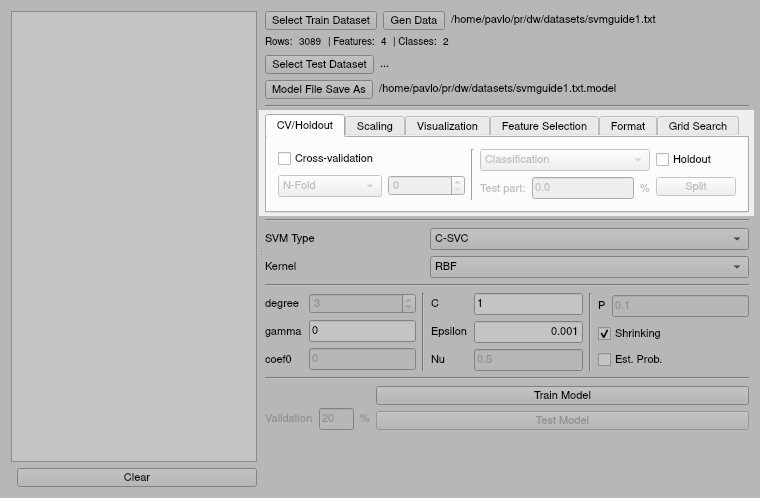
\includegraphics[scale=0.7]{./img/svm_app_cv_holdout.png}
            \caption{Karta z kontrolkami do walidacji krzyżowej i holdout}
            \label{fig:cv_holdout}
        \end{center}
    \end{figure}

    \par Holdout polega na rozdzielaniu zbioru na dane trenujące i dane testujące. Najczęściej
    zbiór danych jest w jednym pliku, natomiast biblioteka \textit{LIBSVM} jest zorganizowana
    tak, że potrzebuje plik z danymi trenującymi i plik z danymi testującymi. Za poprawne
    rozdzielenie danych odpowiadają dwa skrypty w języku Python: h4c.py i h4r.py. Pierwszy
    służy do klasyfikacji i stara się zachować stosunek klas w zbiorze testującym, drugi, z
    kolei, służy do regresji i po prostu wybiera podany procent rekordów tworząc plik z danymi
    do testowania. Na karcie jest umieszczona kontrolka \textit{Combo Box} która pozwala wybrać
    pierwsze(\textit{Classification}) lub drugie(\textit{Regression}) podejścia.

    \begin{figure}[H]
        \begin{center}
            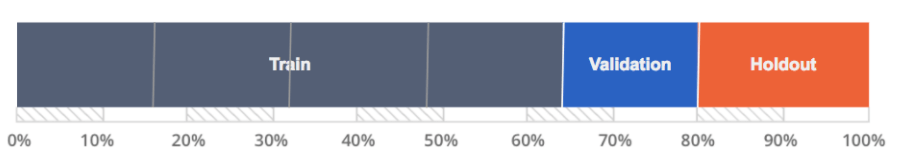
\includegraphics[scale=0.5]{./img/train_validation_holdout.png}
            \captionsource{Przykład podziału zbioru danych. \textit{Train} jest do trenowania,
            a \textit{Holdout} i \textit{Validation} służą do testowania modelu}
            {\url{https://www.datarobot.com/wiki/training-validation-holdout/}}
            \label{fig:tr_val_hl}
        \end{center}
    \end{figure}

    \par Skrypt holdout dla regresji jest również używany w opisanej wyżej walidacji: on
    wybiera losowe rekordy z danych trenujących i tworzy z nich tymczasowy plik testujący na
    którym dalej działa algorytm testowania z biblioteki \textit{LIBSVM}, przez to wynik
    walidacji może się różnić przy takich samych parametrach modelu.

    \par Walidacja krzyżowa jest bardzo ważnym narzędziem w nauczaniu maszynowym. Jeśli danych
    jest mało to rozdzielanie zbioru na dane trenujące i testujące może spowodować
    niedostateczne nauczanie się modelu, w takim przypadku używamy walidacji krzyżowej.
    N-krotna walidacja krzyżowa polega na rozdzielaniu zbioru na N równych części jedna z
    których służy to testowania a wszystkie inne do trenowania. Proces jest iteratywny, więc
    każda część w którejś iteracji będzie służyć do testowania. 

    \begin{figure}[H]
        \begin{center}
            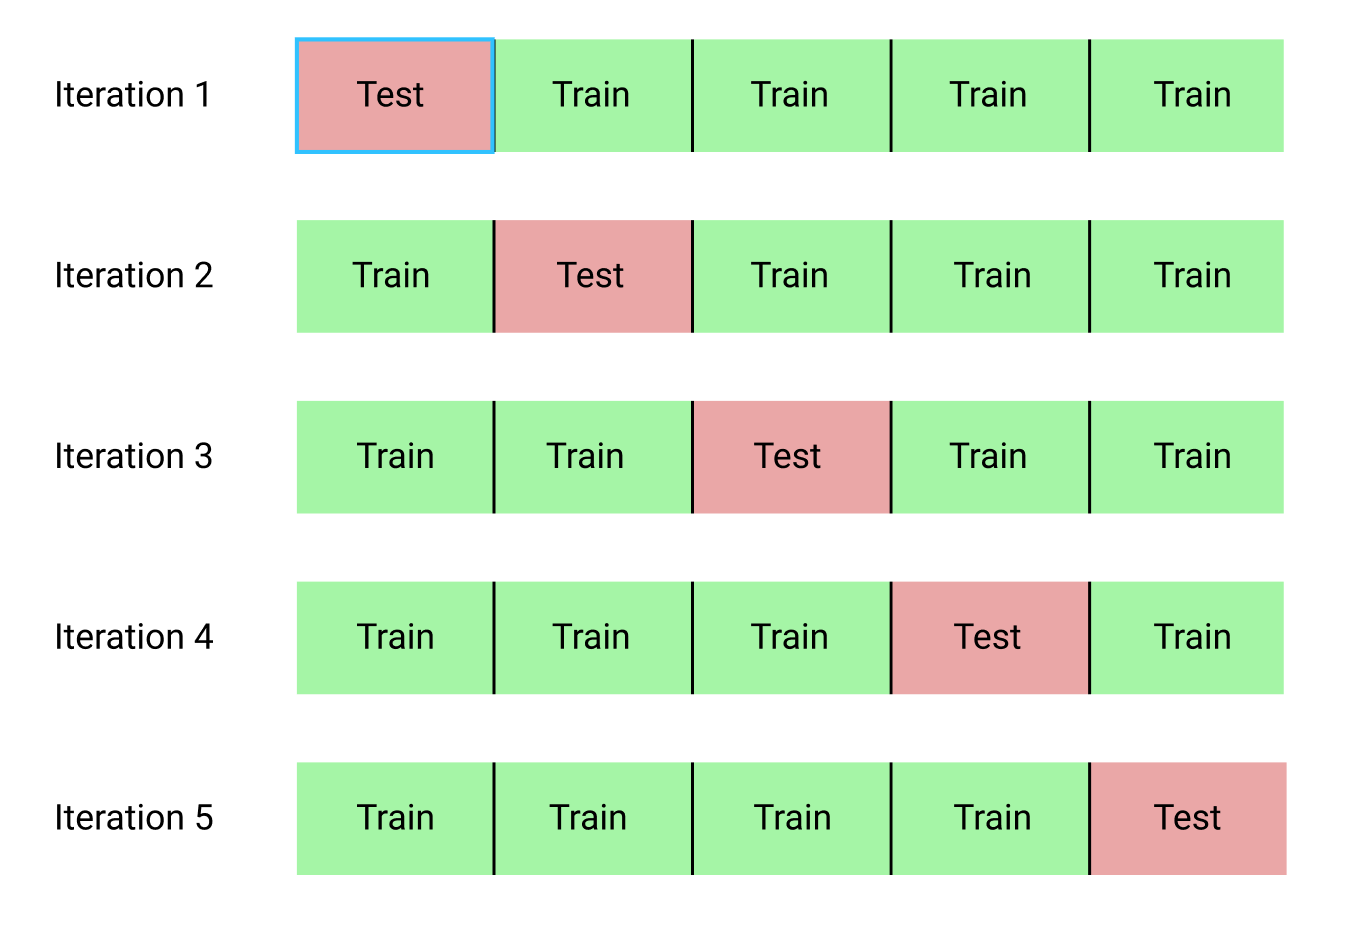
\includegraphics[scale=0.3]{./img/cv_ilustration.png}
            \captionsource{Ilustracja procesu 5-krotnej walidacji krzyżowej}
            {\url{https://towardsdatascience.com/cross-validation-explained-
            evaluating-estimator-performance-e51e5430ff85}}
            \label{fig:cv_ilustr}
        \end{center}
    \end{figure}

    \par Również jest dostępna walidacja krzyżowa typu \textit{Leave-one-out}, która jest
    rodzajem N-krotnej walidacji, tylko zbiór testujący zawsze jest jednoelementowy, czyli jest
    to równoważne podaniu jako N liczby $rozmiar\_zbioru - 1$.
    \par Warto wspomnieć, że walidacja krzyżowa nie generuje modelu, a służy tylko do
    określania jak dobry jest model z podanymi parametrami. Kiedy użytkownik uzna dokładność
    modelu akceptującą on wyłączy walidacje krzyżową i wygeneruje model na całym zbiorze
    trenującym.

\newpage
\subsection{Skalowanie danych}
    \par Karta \textit{Scaling} \ref{fig:scaling} służy do skalowania danych. Główną zaletą
    skalowania danych jest unikanie dominacji cech z większych zakresów liczbowych nad cechami
    z mniejszych zakresów liczbowych. Skalowanie również zmniejsza obciążenie numeryczne dla
    algorytmu, ponieważ funkcje jądrowe często zależą od iloczynu wektorowego lub skalarnego
    cech np.  liniowa i wielomianowa funkcje jądrowe, dla których duże wartości w wektorach
    cech mogą powodować problemy numeryczne.

    \begin{figure}[H]
        \begin{center}
            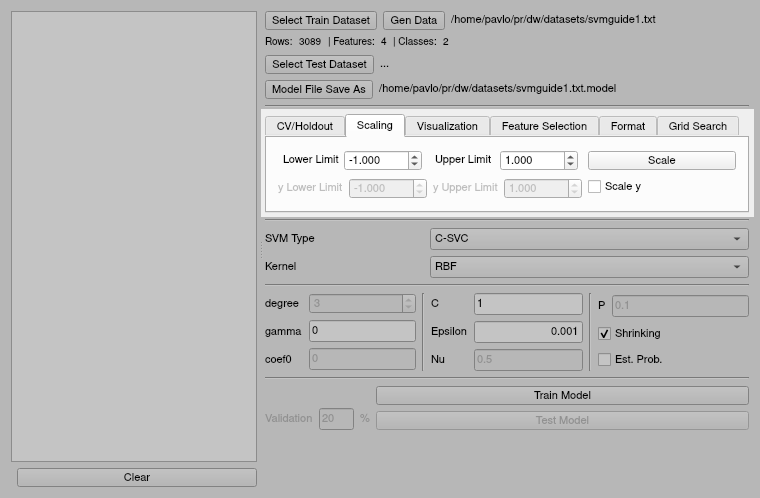
\includegraphics[scale=0.7]{./img/svm_app_scaling.png}
            \caption{Karta z kontrolkami dla skalowania danych}
            \label{fig:scaling}
        \end{center}
    \end{figure}

    \par Twórcy biblioteki \textit{LIBSVM} proponują wszystkim początkującym zaczynać swoją
    pracę z generacją modelu właśnie od skalowania, ponieważ tak prosty krok może mieć bardzo
    wysoki wpływ na dokładność modelu. \\

    \par Przykład wyjścia algorytmu trenującego na tym samym zbiorze danych z takimi samymi
    parametrami do i po skalowaniu danych:
    
    \begin{verbatim}
        ...*..*
        optimization finished, #iter = 5371
        nu = 0.606150
        obj = -1061.528918, rho = -0.495266
        nSV = 3053, nBSV = 722
        Total nSV = 3053
        Accuracy = 66.925% (2677/4000) (classification)
        Validation Accuracy = 99.6769% (617/619) (classification)

            /* moment w którym było przeprowadzone skalowanie danych */

        *
        optimization finished, #iter = 496
        nu = 0.202599
        obj = -507.307046, rho = 2.627039
        nSV = 630, nBSV = 621
        Total nSV = 630
        Accuracy = 96.15% (3846/4000) (classification)
        Validation Accuracy = 95.7997% (593/619) (classification)
    \end{verbatim}
    \par Na tym przykładzie widać, że dokładność modelu wzrosła na 30\% przy dziesięciokrotnym
    zmniejszeniu liczby iteracji algorytmu.\\

    \par Biblioteka \textit{LIBSVM} zawiera w sobie program \textit{svm-scale} który służy do
    poprawnego skalowania danych. W ramach projektu aplikacji kod tego programu został
    przerobiony i zawarty w klasie \textit{svmscale}. Po wybraniu zbioru trenującego kontrolki
    skalowania danych robią się aktywne. Po skalowaniu aplikacja tworzy nowe pliki z danymi
    które kończą się na \textit{.scale}. Warto zauważyć że zbiór trenujący i testujący muszą
    być skalowane razem, a więc przypadek w którym użytkownik wybiera zbiór trenujący, skaluję
    go, wybiera zbiór testujący i przeprowadza skalowanie ponownie może powodować
    nieprzewidywalne konsekwencje. Jeśli użytkownik planuje skalować dane i testować swój model
    to poprawnym podejściem jest wybranie zbiorów danych, a już za tym skalowanie danych.

    \par Również jest dostępne skalowanie klas, które aktywuje się ptaszkiem w polu
    \textit{Scale y}. Może to być przydatne w regresji, kiedy liczby w kolumnie $Y$(kolumna
    klas) nie są dyskretne. Za realizacją skalowania klas stoi wyżej wymieniony program
    \textit{svm-scale}.

\newpage
\subsection{Wizualizacja danych}
    \par Karta \textit{Visualization} \ref{fig:visualization} służy do wizualizacji jedno-,
    dwu- i trzy-wymiarowych danych. 

    \begin{figure}[H]
        \begin{center}
            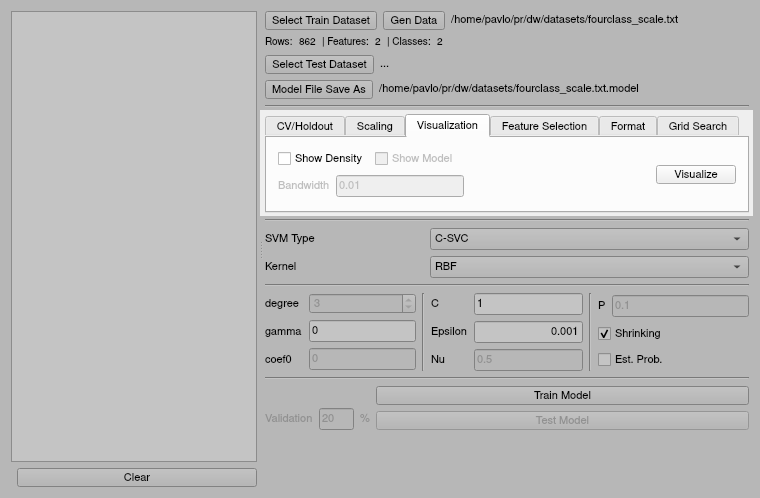
\includegraphics[scale=0.65]{./img/svm_app_visualization.png}
            \caption{Karta z kontrolkami dla wizualizacji danych}
            \label{fig:visualization}
        \end{center}
    \end{figure}

    \par Kontrolki na karcie są dostępne tylko wtedy gdy jest wybrany zbiór trenujący z liczbą
    cech od 1 do 3. 

    \begin{figure}[H]
        \begin{center}
            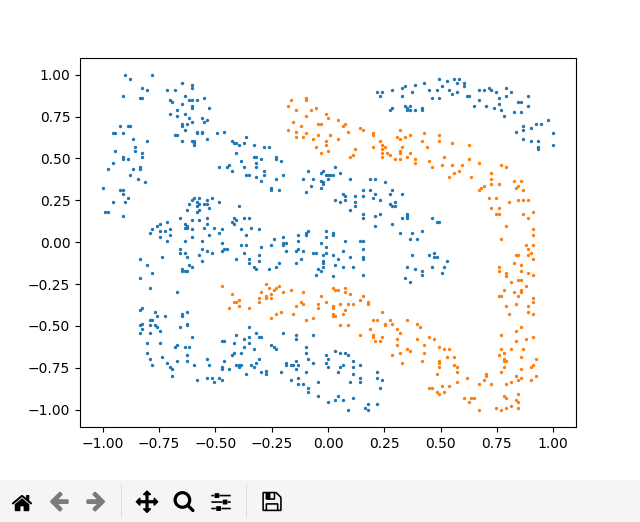
\includegraphics[scale=0.65]{./img/2dplot_ex1.png}
            \caption{Przykład wizualizacji dwuwymiarowych danych}
            \label{fig:visualization}
        \end{center}
    \end{figure}

    \par Dla jedno- i dwu-wymiarowych danych jest dostępne rysowanie gęstości danych. Algorytm
    rysujący dzieli pole wykresu na kwadraty i zlicza liczbę punktów w każdym z nich. Na
    podstawie tego jest generowany konturowy wykres gęstości. Za liczbę kwadratów odpowiada
    wartość \textit{Bandwidth}, która może być ustawiana przez użytkownika na interfejsie
    graficznym. Im mniejszy jest \textit{Bandwidth} tym bardziej gładki wychodzi wykres, ale
    razem z tym zwiększa się obciążenie algorytmu rysującego. 

    \begin{figure}[H]
        \begin{subfigure}{.5\textwidth}
            \centering
            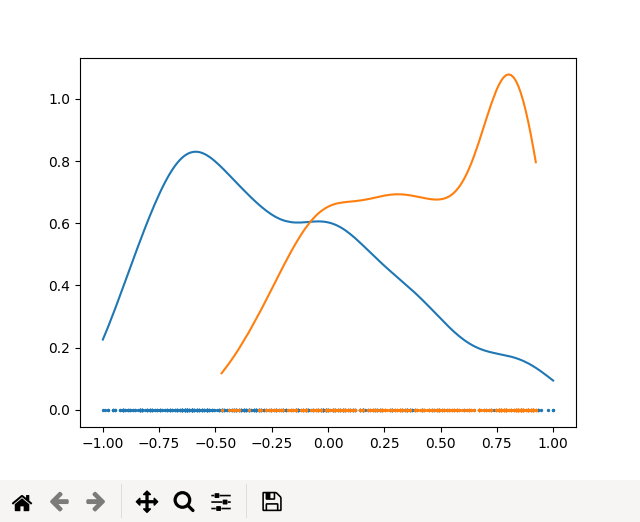
\includegraphics[width=.95\linewidth]{img/1dplot_density.png}
            \label{fig:1dplot_density}
        \end{subfigure}%
        \begin{subfigure}{.5\textwidth}
            \centering
            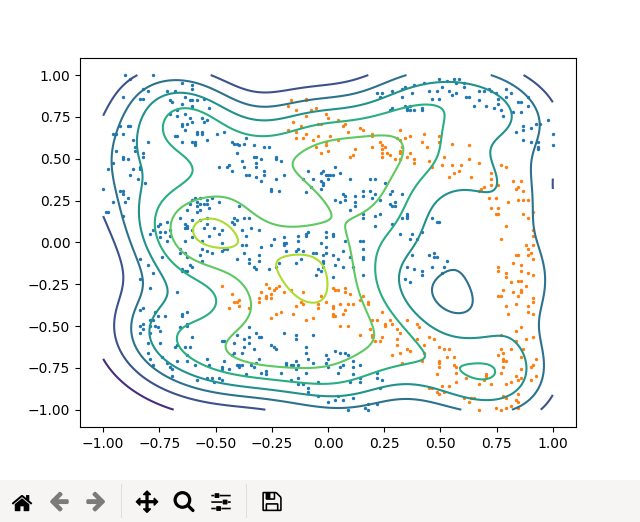
\includegraphics[width=.95\linewidth]{img/2dplot_density.png}
            \label{fig:2dplot_density}
        \end{subfigure}
        \caption{Przykład rysowania gęstości jedno- i dwu-wymiarowych danych}
        \label{fig:density_ex}
    \end{figure}
    
    \par Dla dwuwymiarowych danych jest dostępne rysowanie modelu.

    \begin{figure}[H]
        \begin{center}
            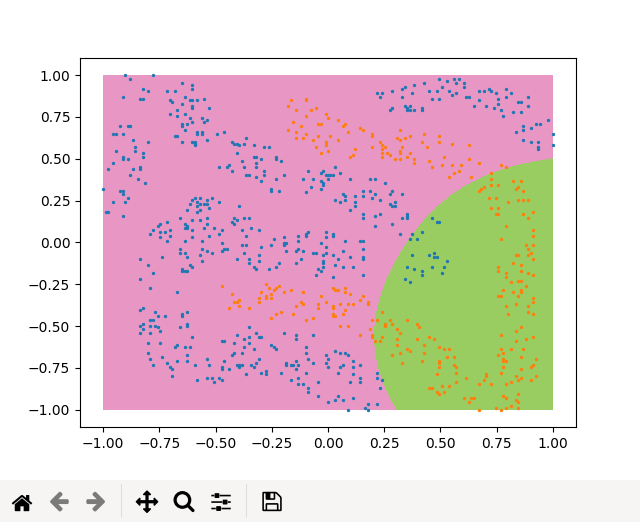
\includegraphics[scale=0.65]{./img/2dplot_model1.png}
            \caption{Przykład rysowania modelu}
            \label{fig:bad_model_visualization}
        \end{center}
    \end{figure}

    \newpage
    \par Dla wyżej narysowanego modelu \ref{fig:bad_model_visualization} już z wykresu widać że
    parametry dobrane kiepsko.  Dobierając odpowiednie parametry i skalując dane można osiągnąć
    lepsze wyniki:

    \begin{figure}[H]
        \begin{center}
            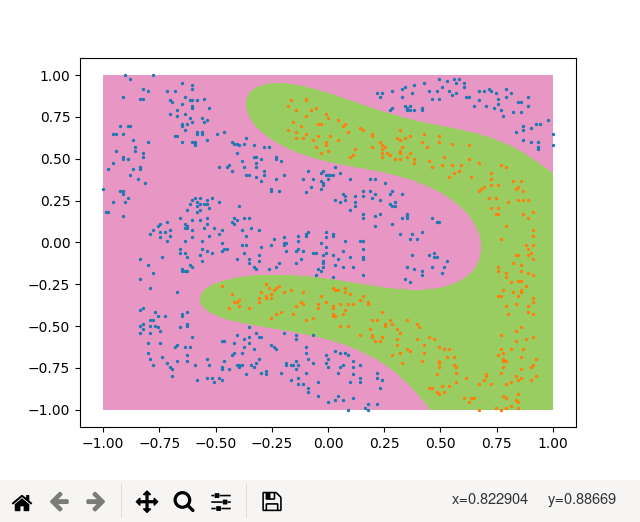
\includegraphics[scale=0.65]{./img/2dplot_model2.png}
            \caption{Przykład rysowania modelu}
            \label{fig:good_model_visualization}
        \end{center}
    \end{figure}

    \par Przycisk \textit{Gen Points} obok kontrolek do wybierania plików z danymi pozwala
    samodzielnie generować zbiór danych. Najpierw trzeba będzie wybrać nazwę pliku i katalog w
    którym należy go umieścić. Za tym pojawi się okno z pustym wykresem, klikając po nim
    użytkownik będzie generował punkty na tej płaszczyźnie, przycisk \textit{Change Group}
    pozwala zmienić klasę aktualnie umieszczanych punktów.

    \begin{figure}[H]
        \begin{center}
            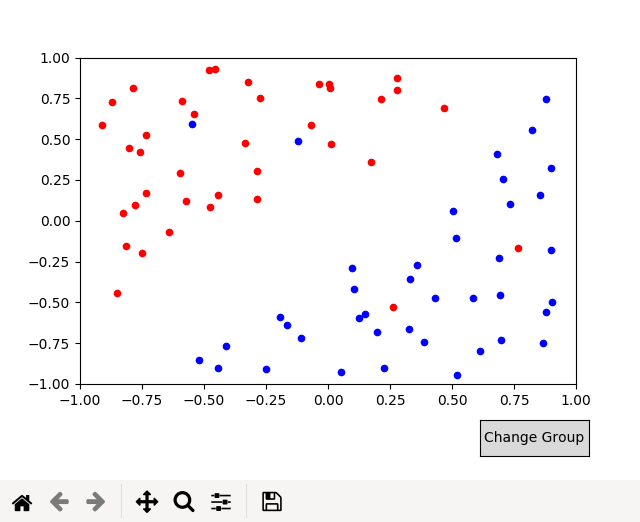
\includegraphics[scale=0.55]{./img/gen_plot.png}
            \caption{Przykład ręcznego generowania danych}
            \label{fig:gen_plot}
        \end{center}
    \end{figure}

    \par Wygenerowany model z liniową funkcją jądrową:

    \begin{figure}[H]
        \begin{center}
            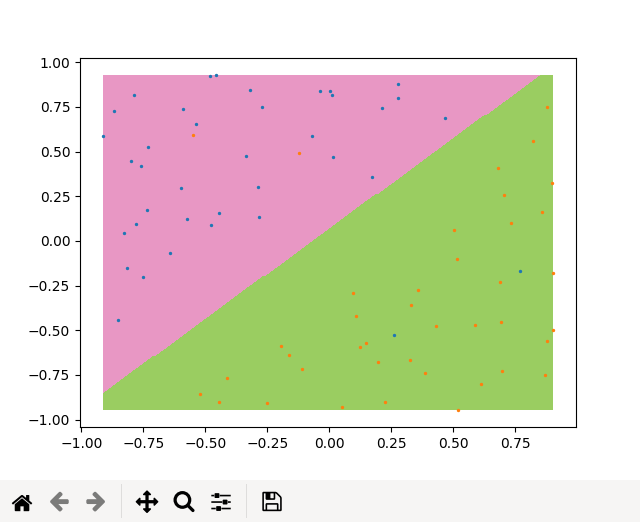
\includegraphics[scale=0.65]{./img/gen_plot_model.png}
            \caption{Model z ręcznie wygenerowanych danych}
            \label{fig:gen_plot_model}
        \end{center}
    \end{figure}

    \par Dla rysowania wykresów był napisany skrypt w języku Python \textit{plotter.py}.
    Wykresy gęstości pomaga rysować funkcja \textit{gaussian\_kde} z biblioteki \textit{scipy}.
    Żeby narysować model skrypt generuje siatkę punktów na całym wykresie zapisuję ich do
    tymczasowego pliku i przekazuje go do programu \textit{svm-predict} z biblioteki
    \textit{LIBSVM}, który w wyniku swojego działania zwraca swoje zgadnięcia odnośnie podanych
    punktów, co pozwala kolorować tło wykresu. Skutkiem takiego podejścia jest 'kąciastość'
    linii rozdzielającej klasy. Wartość \textit{Bandwidth} pozwala kontrolować liczbę punktów w
    generowanej siatce i robić bardziej gładką linie.

\newpage
\subsection{Wybór cech}
    \par Czasami jest potrzeba wybrać tylko niektóre cechy z zbioru danych. Dla takich potrzeb
    w aplikacji istnieje funkcjonalność wyboru cech na karcie \textit{Feature Selection}
    \ref{fig:feature_selection}.

    \begin{figure}[H]
        \begin{center}
            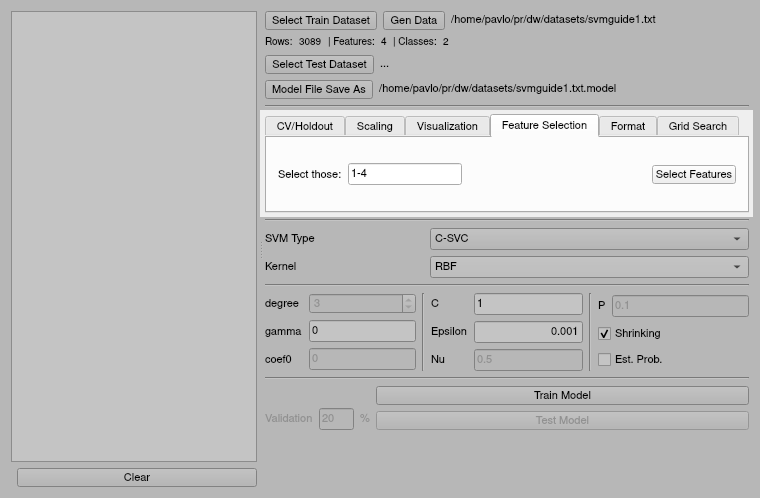
\includegraphics[scale=0.7]{./img/svm_app_fs.png}
            \caption{Karta z kontrolkami do wyboru cech}
            \label{fig:feature_selection}
        \end{center}
    \end{figure}

    \par Na karcie jest umieszczone pole typu \textit{Text Edit}, w które użytkownik musi
    wprowadzić które cechy on chce wybrać. Domyślnie w polu jest wpisany przedział cech w
    wczytanym pliku. Użytkownik może zmienić ten przedział lub wskazać konkretne cechy do
    wyboru, załóżmy że wczytany zbiór danych ma 30 cech, wtedy:

    \begin{verbatim}
    1-10                # wybór cech od 1 do 10
    1-5,10-25           # wybór cech od 1 do 5 i od 10 do 25
    1-5,7,10,15-20,25   # wybór cech od 1 do 5, 7 i 10, od 15 do 20 i 25
    \end{verbatim}

    \par Przycisk \textit{Select Features} uruchamia skrypt w języku Python
    \textit{f\_select.py} który z wybranych zbiorów danych wybiera cechy i zapisuję ich w
    formacie \textit{LIBSVM} do plików z nazwą kończąca się na \textit{.fseleced}. Analogicznie
    do skalowania jeśli użytkownik chce swoje dane testować to przy wyborze cech musi być
    wybrany odpowiedni plik z danymi testującymi.

\subsection{Zmiana formatu danych na \textit{LIBSVM}}
    \par W Internecie trudno znaleźć dane przygotowane w formacie \textit{LIBSVM}, większość z
    nich jest w formacie CSV. Natomiast algorytm trenujący biblioteki \textit{LIBSVM} nie
    przyjmuje danych w innych formatach. Żeby dać swobodę użytkownikom i pozbawić ich od
    potrzeby pisania własnych programów dla konwersji została dodana prosta funkcjonalność
    umieszczona na karcie \textit{Format} \ref{fig:format} pozwalająca konwertować dane do
    formatu \textit{LIBSVM}. Użytkownik musi podać separator pomiędzy cechami i określić czy
    cecha jest na początku lub końcu rekordu. Niestety nie ma opcji żeby liczba określająca
    klasę znajdywała się pomiędzy liczbami oznaczające cechy. Również trzeba określić separator
    dziesiętny liczb rzeczywistych(kropka lub przecinek).

    \begin{figure}[H]
        \begin{center}
            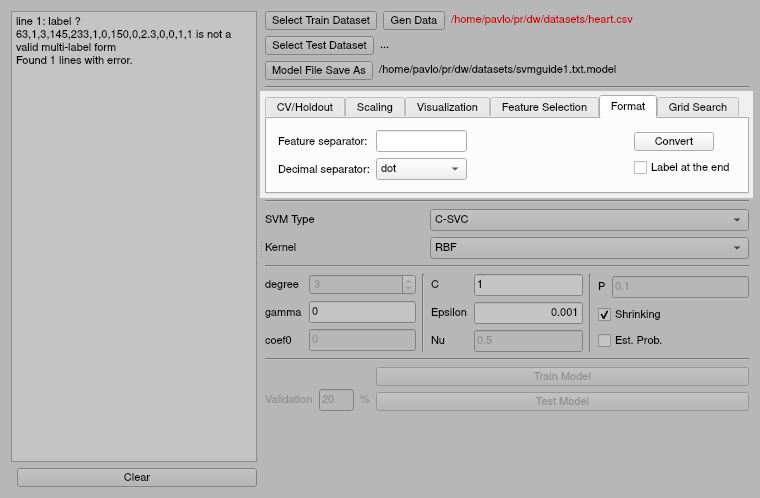
\includegraphics[scale=0.7]{./img/svm_app_format.png}
            \caption{Karta z kontrolkami do formatowania danych}
            \label{fig:format}
        \end{center}
    \end{figure}

    \par Po ustawieniu wszystkich parametrów formatowania i kliknięciu przycisku
    \textit{Convert} aplikacja uruchamia skrypt w języku Python \textit{convert2svm.py} który
    dzięki podanemu separatorowi analizuje podany plik u układa dane w formacie
    \textit{LIBSVM}.

    \par Na przykład to są 5 pierwszych linijek ze zbioru danych w formacie CSV:

    \begin{verbatim}
63,1,3,145,233,1,0,150,0,2.3,0,0,1,1
37,1,2,130,250,0,1,187,0,3.5,0,0,2,1
41,0,1,130,204,0,0,172,0,1.4,2,0,2,1
56,1,1,120,236,0,1,178,0,0.8,2,0,2,1
57,0,0,120,354,0,1,163,1,0.6,2,0,2,1
    \end{verbatim}

    \par Te same dane po formatowaniu(ustawiono flagę że liczby określające klasy są na końcach
    linii):

    \begin{verbatim}
1 1:63 2:1 3:3 4:145 5:233 6:1 7:0 8:150 9:0 10:2.3 11:0 12:0 13:1
1 1:37 2:1 3:2 4:130 5:250 6:0 7:1 8:187 9:0 10:3.5 11:0 12:0 13:2
1 1:41 2:0 3:1 4:130 5:204 6:0 7:0 8:172 9:0 10:1.4 11:2 12:0 13:2
1 1:56 2:1 3:1 4:120 5:236 6:0 7:1 8:178 9:0 10:0.8 11:2 12:0 13:2
1 1:57 2:0 3:0 4:120 5:354 6:0 7:1 8:163 9:1 10:0.6 11:2 12:0 13:2
    \end{verbatim}

\subsection{Optymalizacja parametrów}
    \par Przeszukiwanie siatką(ang. grid search) jest algorytmem pozwalającym na dobór
    parametrów modelu. Biblioteka \textit{LIBSVM} dostarcza skrypt w języku Python
    \textit{grid-search} dla parametrów C i \textit{gamma} który był zintegrowany z aplikacją.
    Probuje on różne kombinacje $(C, \gamma)$(działa w oparciu o funkcje jądrową RBF) i
    wypisuje tą dla której walidacja krzyżowa dała najlepszy wynik. 

    \begin{figure}[H]
        \begin{center}
            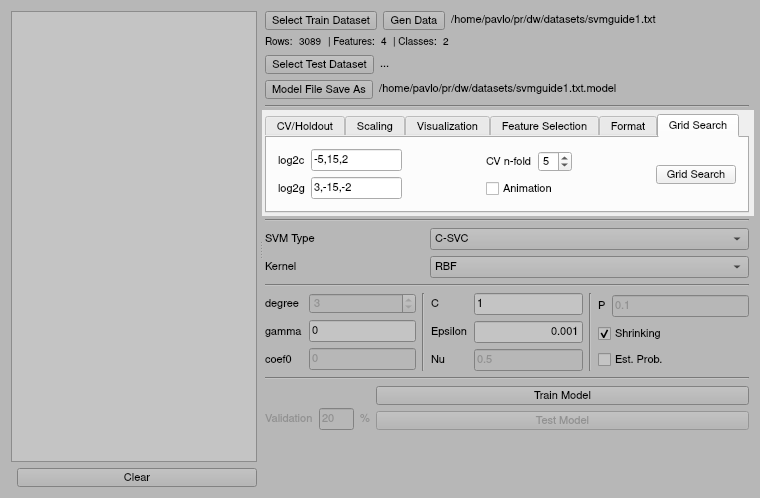
\includegraphics[scale=0.7]{./img/svm_app_grid_search.png}
            \caption{Karta z kontrolkami do przeszukiwania siatką}
            \label{fig:grid_search}
        \end{center}
    \end{figure}

    \par Na karcie \textit{Grid Search} znajdują się dwa pola tekstowych pozwalających na ustawienie
    zakresów parametrów i kroków algorytmu. W pole należy wpisać trzy liczby: początek, koniec
    i krok. Zakres próbowanych parametrów więc będzie wyglądał tak:
    $2^{begin,...,begin+k*step,...end}$. Przeszukiwanie siatką pomaga wybrać potrzebne
    parametry nie zgadując i nie wprowadzając ręcznie każdej pary, wadą jednak jest że proces
    jest dość wolny. 
    \par Na karcie \textit{Grid Search} znajduje się kontrolka typu \textit{Check Box}
    pozwalająca włączyć animacje procesu przeszukiwania jeśli na używanym systemie jest
    skonfigurowana aplikacja \textit{gnuplot}. Również można wybrać krotność walidacji
    krzyżowej używanej dla testowania każdej pary parametrów. 

\subsection{Shrinking \textbf{\textcolor{red}{Kurczenie się????}}}
    \par W sekcji wyboru parametrów trenowania jest umieszczona kontrolka typu \textit{Check
    Box} która pozwala włączyć kurczenie się(ang. shrinking) \textbf{\textcolor{red}{dobre
    tłumaczenie na polski?}} dla algorytmu trenującego. Metoda polega na wyeliminowaniu
    elementów ograniczonych(np. $\alpha_i = 0$ lub $C$) dla zmniejszenia rozwiązywanego
    problemu \cite{CC01a}. 
    \par Kurczenie się nie ma wpływu na dokładność ale pomaga zmniejszyć czas trenowania
    modelu, efekt jest bardziej zauważalny przy dużej liczbie iteracji \cite{libsvm_faq}.

\subsection{Probability estimates}

\newpage
\section{Kompilacja i zależności}
\subsection{Zależności}

    \par Aplikacja była testowana na trzech systemach operacyjnych: \textit{OS X},
    \textit{Debian 10} i \textit{Manjaro Linux 19.0.2}. Lista zależności jest dla systemu
    \textit{Debian 10} skoro jest on najbardziej dostępny i najpopularniejszy z wyżej
    wymienionych.
    \par Zależności systemowe: \textit{git, qt5-default, python3-pip}. Paczki można zainstalować
    poleceniem:

    \begin{verbatim}
    apt-get install git qt5-default python3-pip
    \end{verbatim} 

    lub za pomocą wybranego managera paczek.

    \par Zależności dla \textit{Python 3}: \textit{numpy, scipy, matplotlib}. Paczki można
    zainstalować poleceniem:

    \begin{verbatim}
    pip3 install numpy scipy matplotlib
    \end{verbatim} 

\subsection{Kompilacja}
    \begin{enumerate}
        \item Ściągnąć kod projektu z repozytorium:
        \begin{verbatim}
    git clone https://github.com/boidachenkop/svm-app.git
        \end{verbatim} 

        \item Przejść do katalogu z kodem źródłowym: 
        \begin{verbatim}
    cd svm-app/svm-app
        \end{verbatim} 

        \item Uruchomić kompilacje:
        \begin{verbatim}
    make
        \end{verbatim} 

        \item Skompilawać osobno pliki \textit{svm-train.c} i \textit{svm-predict.c}:
        \begin{verbatim}
    g++ -Wall -Wconversion -O3 -fPIC svm-predict.c svm.o -o svm-predict -lm
    g++ -Wall -Wconversion -O3 -fPIC svm-train.c svm.o -o svm-train -lm
        \end{verbatim} 

    \end{enumerate}

\newpage
\section{Przykłady działania aplikacji} %SECTION
\subsection{Przykład 1}
    \par Przykład pokazujący pracę z plikiem z nieprzeskalowanymi danymi w formacie
    \textit{LIBSVM}

\begin{enumerate}[label={\textbf{Krok \theenumi :}},leftmargin=*]
    \item Wczytać plik z danymi

    \begin{figure}[H]
        \begin{center}
            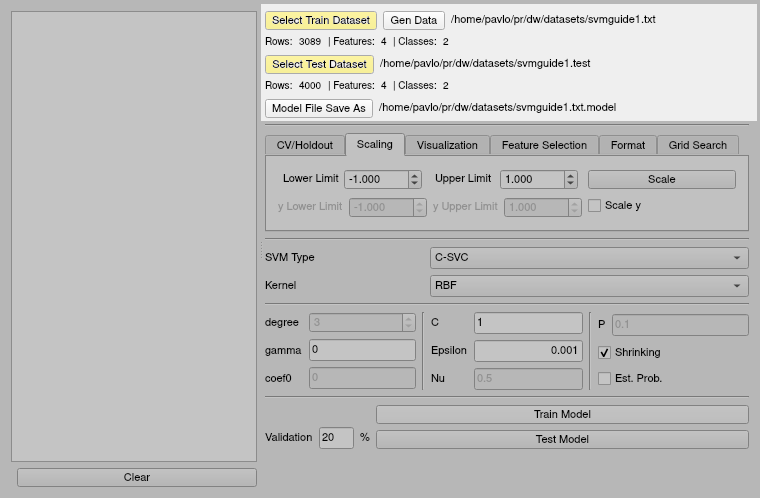
\includegraphics[scale=0.7]{./img/ex1_st1.png}
        \end{center}
    \end{figure}

    Pojawiły się ścieżki z plikami, a pod nimi informacje o wczytanych zbiorach danych,
    więc dane wczytane poprawnie.

    \newpage
    \item Wyskalować dane do przedziału $[-1,1]$

    \begin{figure}[H]
        \begin{center}
            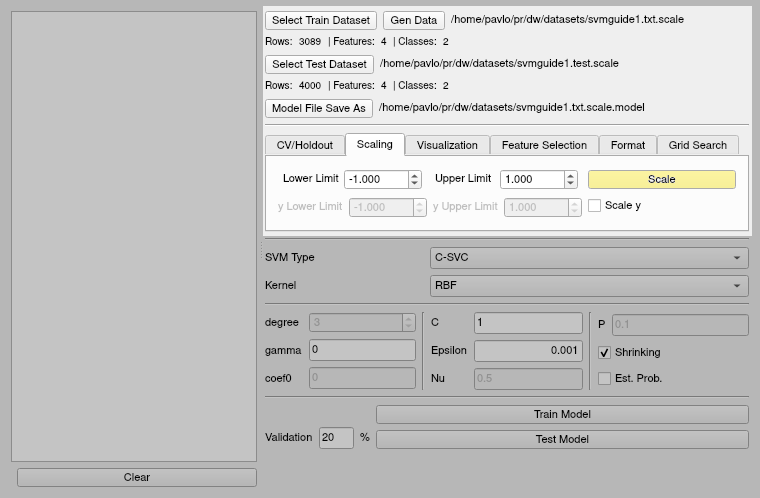
\includegraphics[scale=0.7]{./img/ex1_st2.png}
        \end{center}
    \end{figure}

    Do nazw plików z danymi dodano rozszerzenie \textit{.scale}, więc dane są wyskalowane.

    \item Przeprowadzić przeszukiwanie siatką, żeby dobrać pasujące parametry.

    \begin{figure}[H]
        \begin{center}
            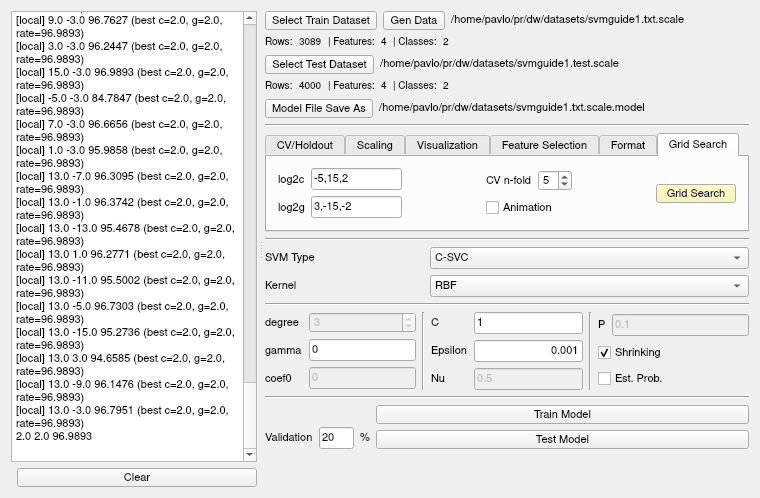
\includegraphics[scale=0.7]{./img/ex1_st3.png}
        \end{center}
    \end{figure}

    Algorytm przeszukiwania siatką zwrócił że przy parametrach $C=2$, $gamma=2$ precyzja modelu
    będzie około 96\%.

    \item Wytrenować i przetestować model dla parametrów zwróconych algorytmem optymalizującym.

    \begin{figure}[H]
        \begin{center}
            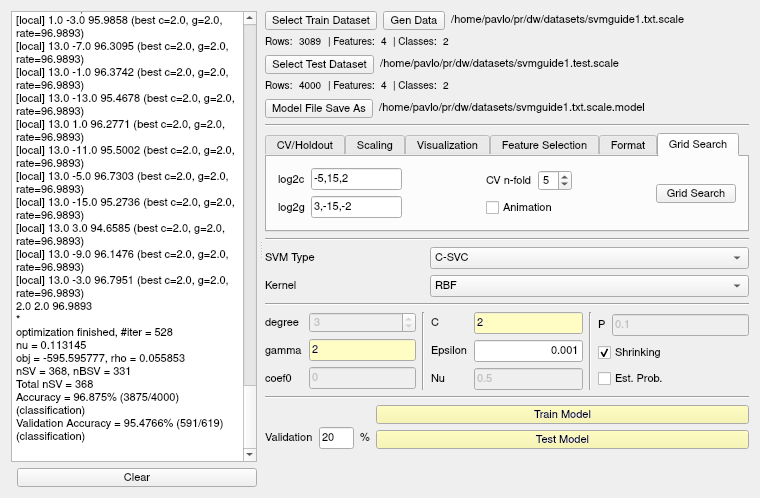
\includegraphics[scale=0.7]{./img/ex1_st4.png}
        \end{center}
    \end{figure}

    Wytrenowany model znajduje się w ścieżce podanej naprzeciwko przycisku \textit{Model File
    Save as}. 
\end{enumerate}

\newpage
\subsection{Przykład 2}
    \par Przykład z danymi w formacie \textit{CSV}. 
\begin{enumerate}[label={\textbf{Krok \theenumi :}},leftmargin=*]

    \item Wczytać plik z danymi.
    \begin{figure}[H]
        \begin{center}
            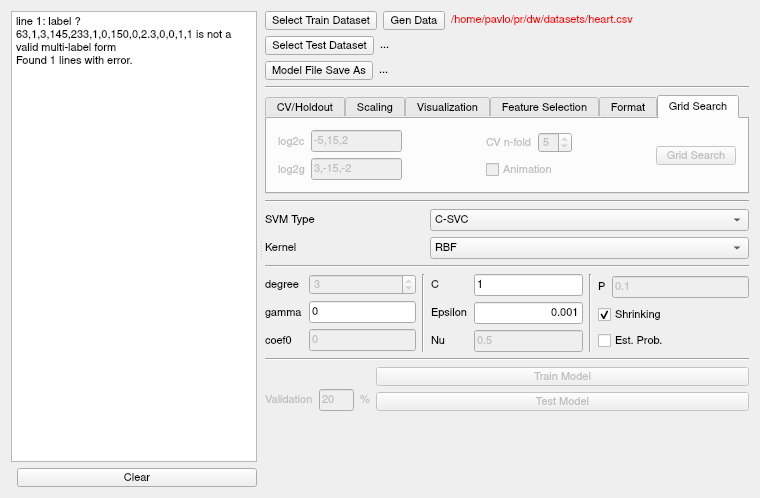
\includegraphics[scale=0.7]{./img/ex2_st1.png}
        \end{center}
    \end{figure}

    Ścieżka do wczytanego pliku jest czerwonego koloru, co sygnalizuje o błędzie, komunikat w
    polu tekstowym mówi że wczytane dane nie są w formacie \textit{LIBSVM}.

    \item Skonwertować dane do formatu \textit{LIBSVM}.

    \begin{figure}[H]
        \begin{center}
            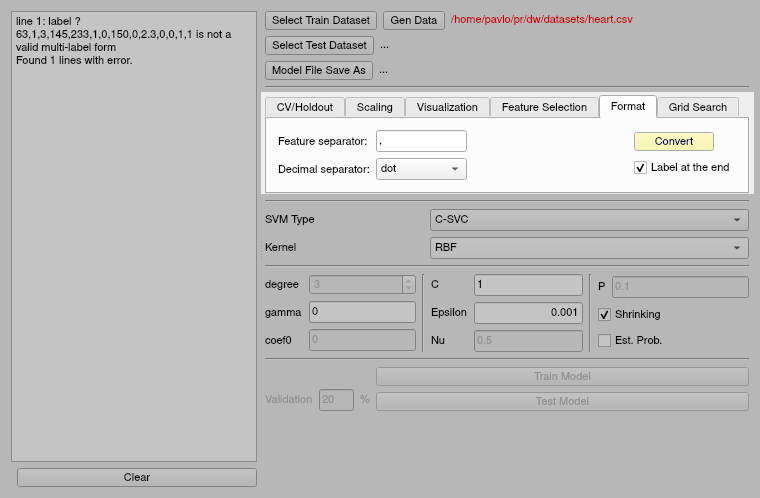
\includegraphics[scale=0.7]{./img/ex2_st2.png}
        \end{center}
    \end{figure}

    Należy wprowadzić separator danych i zaznaczyć ptaszkiem czy liczba wskazująca klasę jest
    na początku lub końcu linii. W danym przypadku separatorem jest przecinek, a kolumna klas
    jest na końcu. Po kliknięciu na przycisk \textit{Convert} program automatycznie wczyta plik
    z skonwertowanymi danymi i wypisze informację o nich.
    
    \item Wyskalować dane do przedziału $[-1, 1]$.

    \begin{figure}[H]
        \begin{center}
            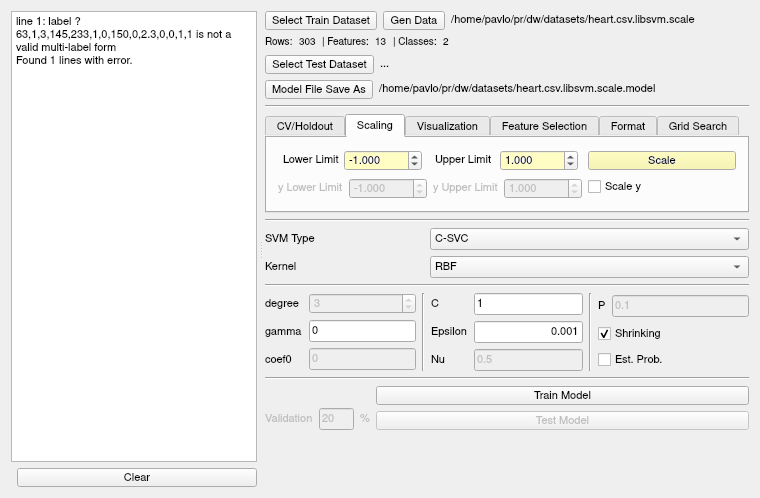
\includegraphics[scale=0.7]{./img/ex2_st3.png}
        \end{center}
    \end{figure}

    Skoro w danym zbiorze jest tylko 303 rekordy nie będziemy dzielić go na zbiór testujący i
    trenujący, a użyjemy walidacji krzyżowej. Do nazwy pliku z danymi było dodane
    \textit{.scale}, więc dane są wyskalowane.

\newpage
    \item Uruchomić przeszukiwanie siatką, żeby dobrać odpowiednie parametry.

    \begin{figure}[H]
        \begin{center}
            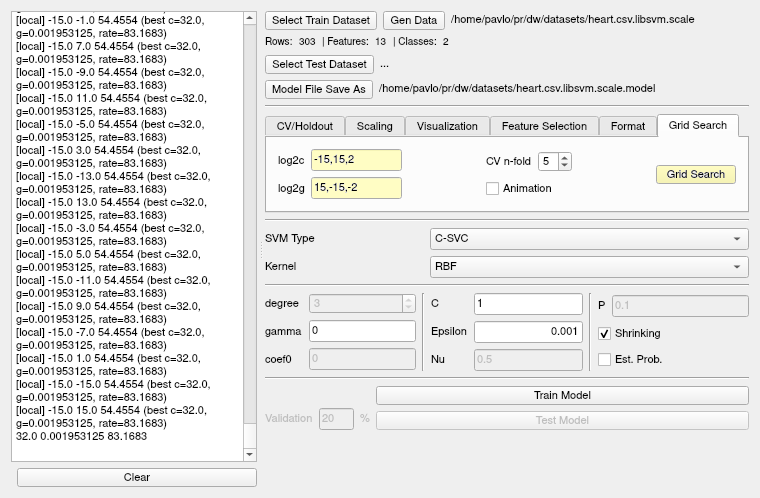
\includegraphics[scale=0.7]{./img/ex2_st4.png}
        \end{center}
    \end{figure}

    Algorytm zwrócił parametry $C=32$, $gamma=0.001953$ na których 5-krotna walidacja
    krzyżowa pokazuje precyzje modelu w 83\%. Mając bardziej szczegółową wiedze o tym zbiorze
    danych np. co reprezentują cechy można było by spróbować wyrzucić te które nie dotyczą
    rozwiązywanego zadania i uzyskać większą dokładność modelu.

    \item Wygenerować model.

    \begin{figure}[H]
        \begin{center}
            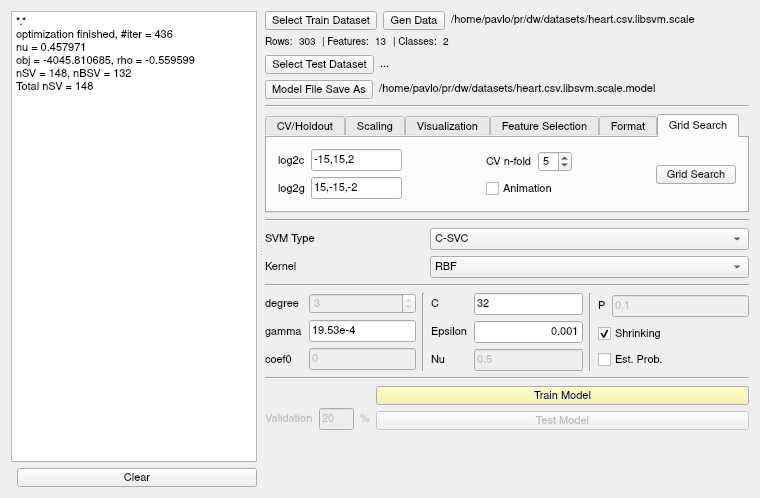
\includegraphics[scale=0.7]{./img/ex2_st5.png}
        \end{center}
    \end{figure}

\end{enumerate}

\subsection{Przykład 3}
    \par Przykład reprezentujący pracę z ręcznie wygenerowanymi danymi.

\begin{enumerate}[label={\textbf{Krok \theenumi :}},leftmargin=*]
    \item Wcisnąć przycisk \textit{Gen Data} i wybrać lokalizację i nazwę dla pliku z ręcznie
        wygenerowanymi danymi.

    \begin{figure}[H]
        \begin{center}
            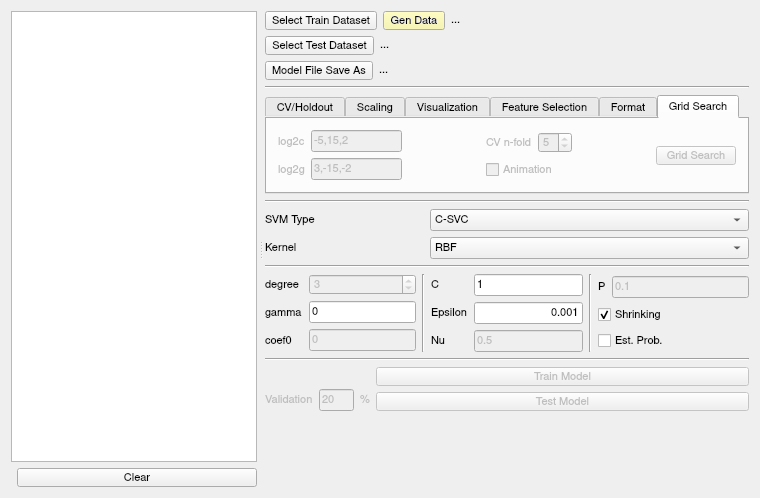
\includegraphics[scale=0.7]{./img/ex3_st1.png}
        \end{center}
    \end{figure}

    \newpage
    \item Klikając na płaszczyźnie generować punkty. Dla zmiany klasy należy kliknąć w przycisk
        \textit{Change Group}.

    \begin{figure}[H]
        \begin{center}
            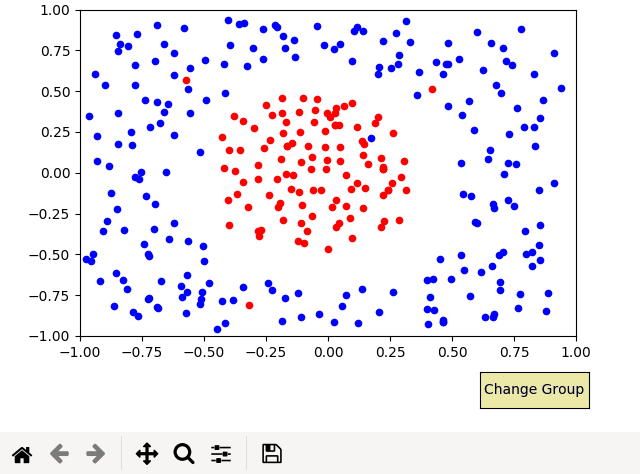
\includegraphics[scale=0.6]{./img/ex3_st2.png}
        \end{center}
    \end{figure}

    Staram się imitować klasyczny przykład na którym jest pokazywane działanie funkcji
    jądrowych. W kolejnym kroku nie ma potrzeby skalować dane skoro granice płaszczyzny na
    której generujemy dane są w przedziałach $x\in [-1, 1]$ i $y\in [-1, 1]$

    \item W celu zadowolenia interesu użyjmy liniowej funkcji jądrowej z domyślnymi
        parametrami.

    \begin{figure}[H]
        \begin{center}
            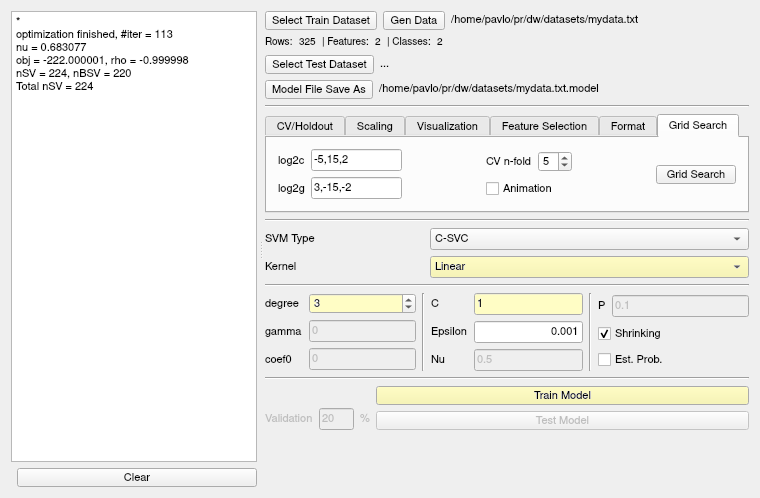
\includegraphics[scale=0.7]{./img/ex3_st3.png}
        \end{center}
    \end{figure}

    \newpage
    \item Po wygenerowania modelu można zwizualizować go.

    \begin{figure}[H]
        \begin{center}
            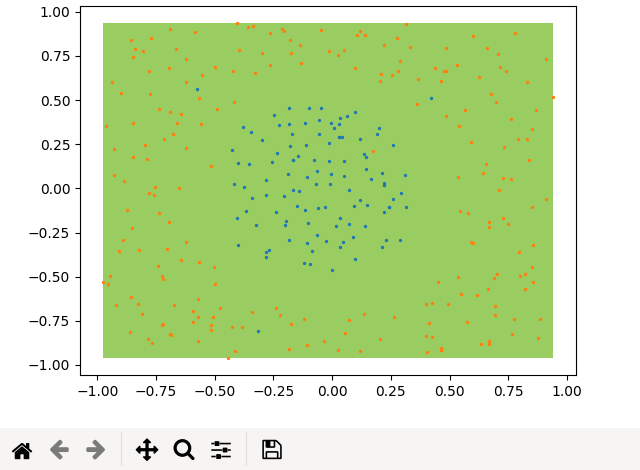
\includegraphics[scale=0.7]{./img/ex3_st4.png}
        \end{center}
    \end{figure}

    Algorytm \textit{SVM} przydzielił wszystkie punkty do jednej klasy i według 5-krotnej
    walidacji krzyżowej uzyskał precyzje 65.84\%. Jest to, oczywiście, kiepski model.
    
    \item Wróćmy do funkcji jądrowej RBF i spróbujmy uruchomić przeszukiwanie siatką.

    \begin{figure}[H]
        \begin{center}
            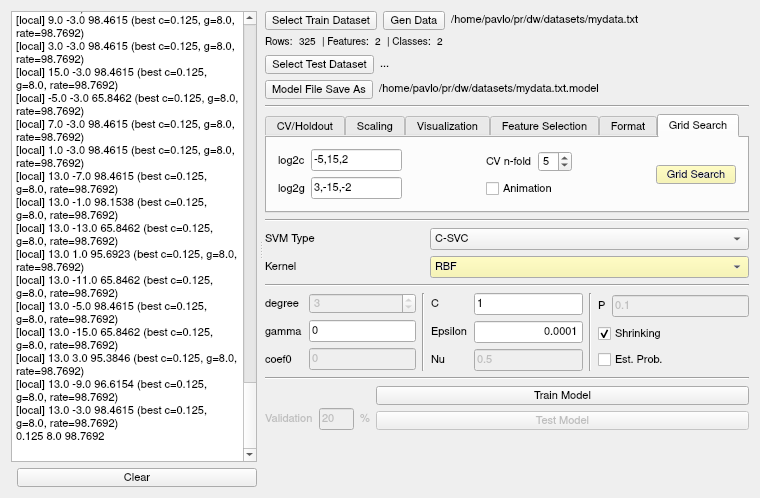
\includegraphics[scale=0.66]{./img/ex3_st5.png}
        \end{center}
    \end{figure}

    Algorytm proponuje użyć parametrów $C=0.125$ i $gamma=8$ dzięki którym potrafimy uzyskać
    znacznie lepszą precyzje: 98.76\%!

    \newpage
    \item Po wygenerowaniu modelu można go zwizualizować.

    \begin{figure}[H]
        \begin{center}
            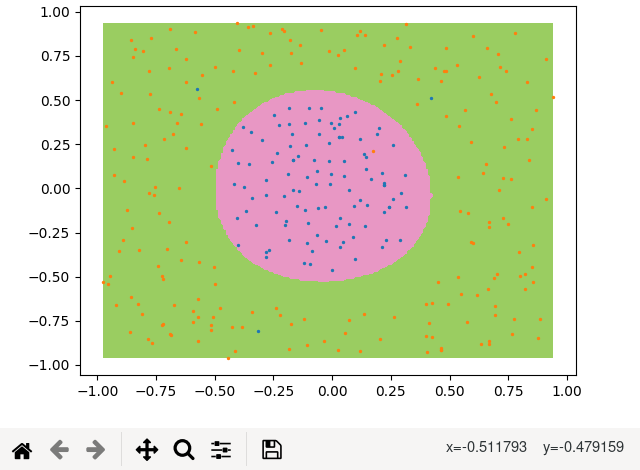
\includegraphics[scale=0.69]{./img/ex3_st6.png}
        \end{center}
    \end{figure}

    Z wykresu widać że ten model jest znacznie lepszy. Algorytm poprawnie zidentyfikował
    szumy(punkty znajdujące się pomiędzy punktami z innej klasy) i nie widać przeuczania. 


\item W celach zadowolenia interesu sprobujmy sztucznie wywołać zjawisko przeuczania, np.
    podając jako parametry $C=500$ i $gamma=20$. Po wygenerowaniu modelu będzie on miał
    taki wygląd.

    \begin{figure}[H]
        \begin{center}
            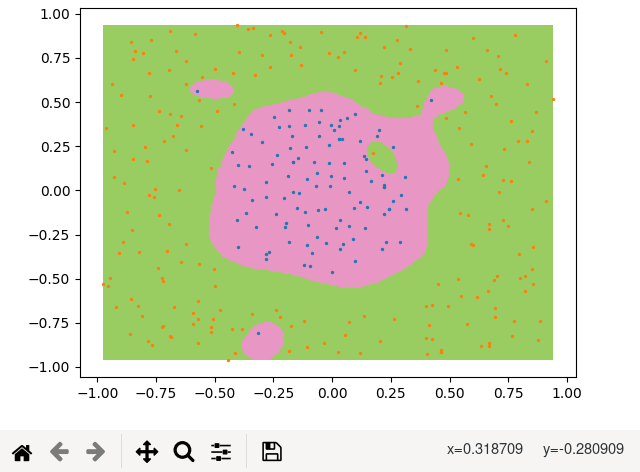
\includegraphics[scale=0.69]{./img/ex3_st7.png}
        \end{center}
    \end{figure}

    W tym przypadku model bierze pod uwagę punkty które były wprowadzone specjalnie w roli
    szumów, 5-krotna walidacja krzyżowa zwraca gorszy wynik: 95.69\%

\end{enumerate}

\subsection{Przykład 4}
    \par Przykład opisujący prace z zbiorem danych pokazanym na rysunkach
    \ref{fig:bad_model_visualization} i \ref{fig:good_model_visualization}.

    \begin{enumerate}[label={\textbf{Krok \theenumi :}},leftmargin=*]

        \item Wczytać plik \textit{fourclas\_scale.txt} i wytrenować model z domyślnymi
            parametrami.

        \begin{figure}[H]
            \begin{center}
                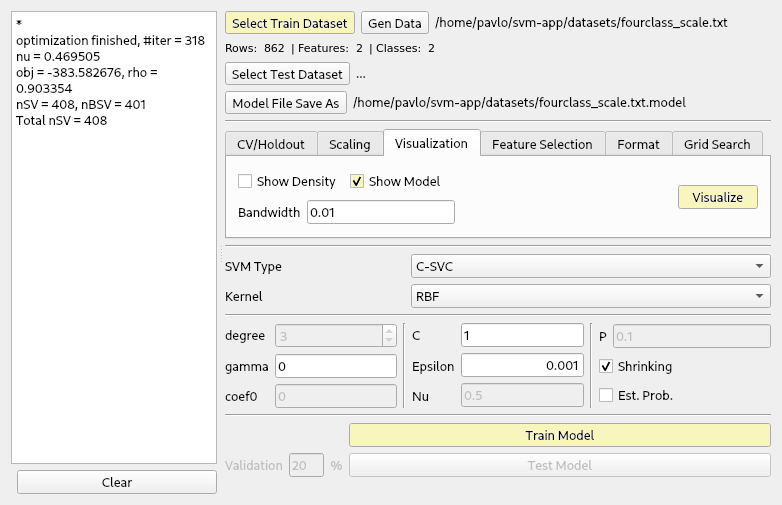
\includegraphics[scale=2.3]{./img/ex4_st1.png}
            \end{center}
        \end{figure}

        \item Zwizualizować model.

        \begin{figure}[H]
            \begin{center}
                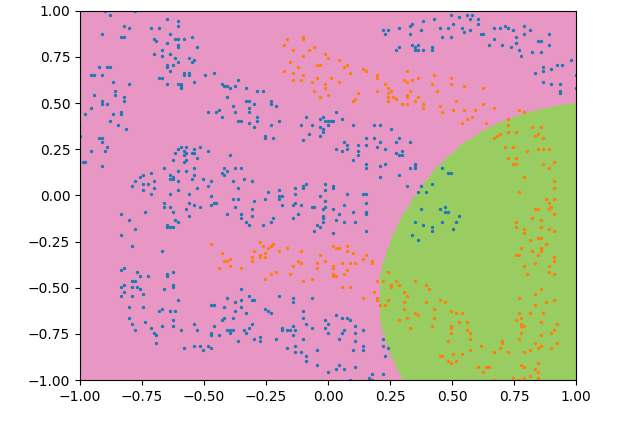
\includegraphics[scale=2.3]{./img/ex4_st2.png}
            \end{center}
        \end{figure}

        \par Widać że parametry dobrane kiepsko, trzeba znaleźć lepsze...

        \newpage
        \item Uruchomić przeszukiwanie siatką(ang. Grid Search) żeby znaleźć lepsze parametry
            dla trenowania.

        \begin{figure}[H]
            \begin{center}
                \includegraphics[scale=2.3]{./img/ex4_st3.png}
            \end{center}
        \end{figure}

        Algorytm zwrócił parametry $C=32.0$, $gamma=2.0$ dla których walidacja krzyżowa dała
        wynik w 100\%.

    \item Wytrenować i zwizualizować model dla znalezionych parametrów.

        \begin{figure}[H]
            \begin{center}
                \includegraphics[scale=2.3]{./img/ex4_st4.png}
            \end{center}
        \end{figure}

        \par Wizualnie widać że klasy są odseparowane lepiej.

    \end{enumerate}
    
\newpage
\section{Podsumowanie} % SECTION
\subsection{Odniesienie do celu pracy}
    \par W ramach pracy udało się stworzyć aplikację z interfejsem graficznym, która potrafi
    trenować i testować modeli, wizualizować dane i wytrenowany model, skalować i przekształcać
    dane. Program może być przydatny dla osób chcących szybko przetestować kilka modeli z
    różnymi parametrami. Przez możliwość wizualizacji modelu aplikacja może być szczególnie
    przydatna w celach dydaktycznych.

\subsection{Rozwój aplikacji}
    \par Jeśli do aplikacji w przyszłości będzie dodawana nowa funkcjonalność to w każdym
    przypadku będzie konieczna zmiana schematu interfejsu graficznego. W trakcie pracy dodając
    nową funkcjonalność tworzyłem nową kartę na której umieszczałem odpowiednie kontrolki,
    kontynuacja tego może spowodować zaśmiecanie interfejsu przez co użytkownikom będzie trudno
    znaleźć kontrolki i meni których potrzebują. Obecnie aplikacja używa jednego okna za
    wyjątkiem okien systemowych dla wyboru plików i okien do wizualizacji danych, rozwiązaniem
    zaśmiecania interfejsu może być użycie wielu okien. Na przykład osobne okno do wizualizacji
    danych, okno dla pracy z plikami i danymi, okno do trenowania i testowania modelu itp. Innym
    podejściem które wydaje się sensownym - praca w jednym oknie, ale zmiana jego treści w
    zależności od akcji użytkownika. Wadą, oczywiście, będzie to że użytkownik zobaczy dostępne
    kontrolki dopiero po akcji(np kontrolki do wizualizacji nie są umieszczane na ekranie do
    wczytania plików z danymi), przez co trudno będzie planować swoją prace. 

    \par W przyszłości warto dodać wstępnie obliczone funkcje jądrowe(ang. \textit{Precomputed
    kernel}). Biblioteka \textit{LIBSVM} ma taką funkcjonalność, natomiast nie została ona
    zaimplementowana w obecnej wersji aplikacji. Polega ona na tym, że wartości funkcji jądrowej
    znajdują się w pliku trenującym.

    \par W nauczaniu maszynowym dane często nie są zbalansowane czyli jedna klasa występuje
    częściej od innej. W przyszłości warto dodać funkcjonalność którą oferuje \textit{LIBSVM}:
    ustawianie wag dla poszczególnych klas, co pozwala walczyć z niezbalansowanymi danymi. 

    \par Podział na pliki trenujące i testujące był zaimplementowany żeby odwzorować działanie
    biblioteki \textit{LIBSVM}, natomiast w rzeczywistości użytkownik najczęściej ma jeden
    plik z danymi. Aplikacja może działać z jednym plikiem, używając walidacji krzyżowej lub
    wyboru danych do testowania z pliku trenującego(ang. \textit{Holdout}), ale wydaje się
    sensowniejszym zrezygnować z założenia że użytkownik ma dwa pliki(testujący i trenujący) na
    korzyść założenia że użytkownik po prostu ma jakiś zbiór danych, nie koniecznie w formacie
    \textit{LIBSVM}.

    \par Istniejący konwerter danych do formatu \textit{LIBSVM} jest bardzo naiwny, i zakłada
    że dane mają separator, a liczba oznaczająca klasę jest na początku lib końcu linii. W
    przyszłości warto zbadać najpopularniejsze formaty do zapisu danych i upewnić się że
    zaimplementowany konwerter sobie z nimi poradzi.

    \par Na obecną chwile aplikacja nie umie pracować z danymi w tekstowej postaci, w
    przyszłości warto to dodać. 

    \par Warto przerobić system wątków i uruchamiania skryptów. Teraz jest tak, że skrypty w
    języku \textit{Python} uruchamiają się na tym samym wątku na którym jest obliczany
    interfejs graficzny, czyli w trakcie działania skryptu interfejs jest zamrażany. W
    przypadku skryptów które działają szybko(np. sprawdzenie poprawności danych) to nie ma
    znaczenia, użytkownik po prostu nie zauważy tego, natomiast skrypt przeszukiwania siatką
    może trwać dość długo(około 30-40 sekund). Tak długa nieaktywność interfejsu może
    naprowadzić użytkownika na myśl, że program się zawiesił i przestał działać. Rozwiązaniem
    może być uruchamianie skryptów w osobnych wątkach, a na interfejsie graficznym umieszczenie
    animacji oznaczającej że program coś liczy i nie trzeba go przerywać. 
    
    \par Można pomyśleć nad dodaniem innych bibliotek w oparciu o które może działać aplikacja,
    pozwoliło by to użytkownikom porównywanie wydajności różnych implementacji \textit{SVM}.

    \par Program ma dość sporo zależności dla uruchamianych skryptów. Należałoby
    zaimplementować system sprawdzający czy wszystkie zależności są zainstalowane i czy
    wszystkie skrypty są w katalogu roboczym.
     

\newpage
\nocite{*}
\printbibliography[title={Źródła}]

\end{document}
